%----------------------ANFORDERUNGSANALYSE-------------------
\chapter{Anforderungsanalyse}
\label{cha:anforderungsanalyse}

In diesem Kapitel wird mit \autoref{sec:ausgangslage} zunächst das bisherige System beschrieben. Mit den anschließenden Abschnitten \ref{sec:anforderungFunktionUndAufbau} bis \ref{sec:anforderungBestellstystem} werden die Anforderungen an das neue, digitale Transportsystem definiert. 

\section{Ausgangslage}
\label{sec:ausgangslage}
Die Gartenhochbahn stellt ein Transportsystem für Essen und Getränke dar. Hauptbestandteil des Systems ist eine Gondel, die sich mit Laufrädern auf einer Schiene fortbewegt. In \autoref{pic:oldhochbahn} ist die Gondel im initialen Zustand dargestellt. An dem Aufbau ist mit Ketten das Tablet befestigt, auf dem Speisen und Getränke abgestellt werden können.  

%@Moritz: Bitte noch Bild mit besserer Auflösung reinmachen.
\begin{figure}[h]
	\begin{center}
		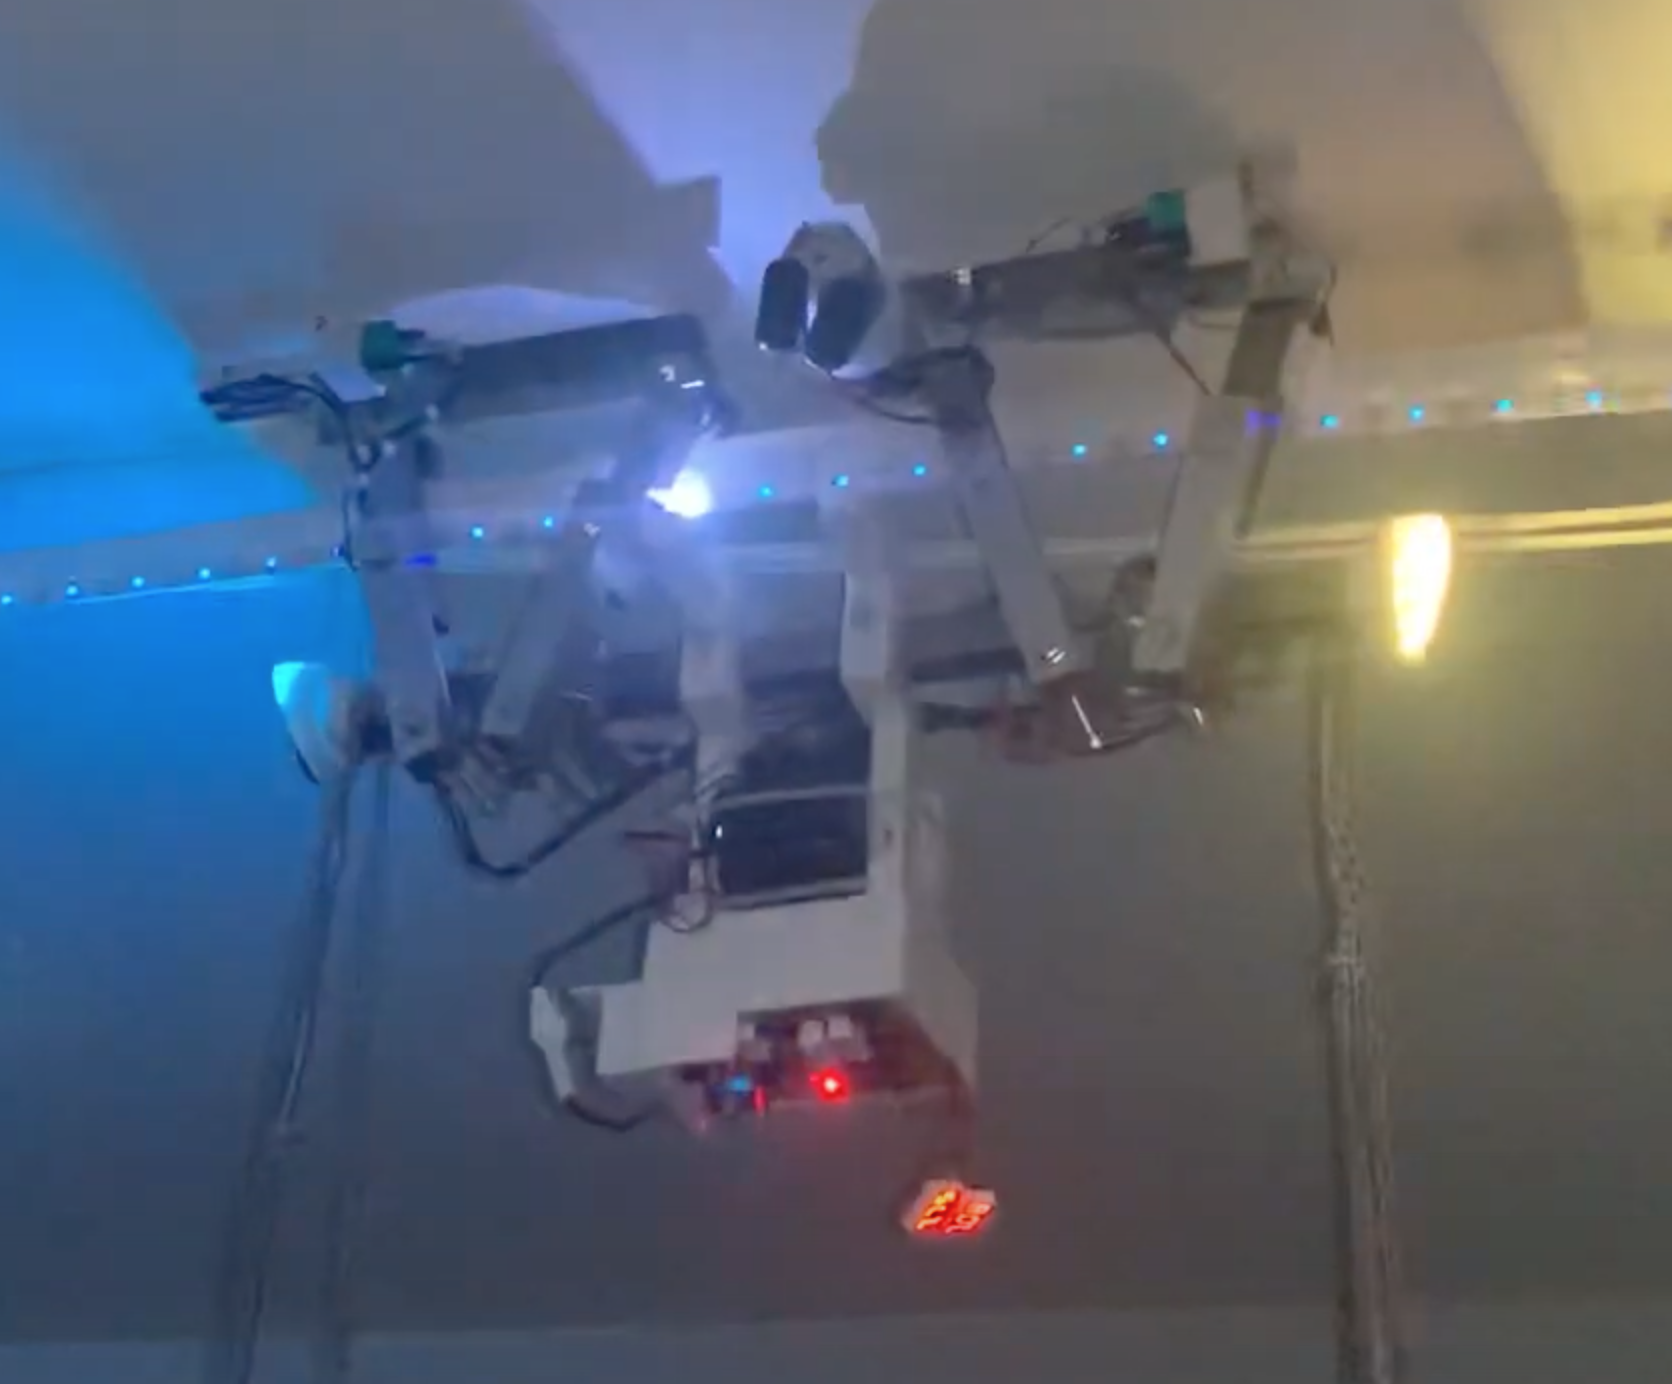
\includegraphics[width=8cm]{oldHochbahn.png}
		\caption{Initialzustand der Gondel}
		\label{pic:oldhochbahn}
	\end{center}
\end{figure}
\newpage

Der Antrieb der Gondel erfolgt mit einem Gleichstrommotor, der mit \acrfull{pwm} angesteuert wird. Die Kraftübertragung auf das treibende Laufrad erfolgt reibschlüssig. Für die Bereitstellung der Energie ist eine Batterie in der Gondel installiert. Diese wird in der Parkstellung am Ende der Schiene aufgeladen. Als Abschaltung des Motors an den hinteren Endlagen sind Tastsensoren verbaut. Ein \acrshort{reed}-Kontakt in der Gondel erkennt außerdem Magnete entlang der Strecke. Nach Erfassen eines Kontaktes an einer Endlage wird die Geschwindigkeit langsam reduziert. Für die Signalverarbeitung und Steuerung des Motors ist ein Arduino Nano im Einsatz. \\

Mit drei Tastern können verschiedene Stationen auf dem Weg angefahren werden. Damit ist ein einzelner Fahrzyklus bereits automatisiert. Ziel dieses Projektes ist es, den gesamten Bestellprozess mit Liefervorgang zu automatisieren. \\

Der bisherige Gondelaufbau entspricht in vielen Punkten nicht den Anforderungen. Dazu zählt vor allem der hohe Verschleiß des reibschlüssigen Antriebs. Da der initiale Aufbau in grundlegenden Punkten verändert werden müsste, wird im Rahmen des Projektes die Gondel neu aufgebaut. In den folgenden Abschnitten werden Anforderungen an die neue Gondel gestellt. 

\section{Funktion und Aufbau}
\label{sec:anforderungFunktionUndAufbau}
Der Aufbau soll dafür ausgelegt sein, Getränke und Speisen bis zu einem Gewicht von $\approx$5Kg zu transportieren. Um die Bestellung unversehrt liefern zu können, darf ein bestimmter Neigungswinkel nicht überschritten werden. Zu diesem Zweck muss das Kippmoment der Gondel abgefangen werden. Auf den Schienen muss sich die Gondel selbst bei engen Radien zuverlässig fortbewegen können. Damit die Entladespannung der Batterie nicht unterschritten wird, muss diese überwacht werden. Wird eine bestimmte Spannungsschwelle unterschritten, soll ein Zurückfahren in die Ladestation erzwungen werden. Da der größte Teil der Hochbahn überdacht ist, muss keine Rücksicht auf Witterungsbedingungen genommen werden. Die Konzeptionierung des Aufbaus erfolgt in \autoref{sec:konzeptGrundaufbau}.
\newpage


\section{Antrieb}
\label{sec:anforderungAntrieb}
Insgesamt soll der Antrieb eine hohe Zuverlässigkeit aufweisen und verschleißarm sein. 
Die Kraftübertragung soll mit einer passenden Übersetzung erfolgen. Durch den elektrischen Motor soll eine Regelung der Geschwindigkeit und Drehrichtung möglich sein. Wünschenswert wäre außerdem eine Rückmeldung der Umdrehungen. Beim Beschleunigen und Bremsen darf nichts von den Speisen und Getränken verschüttet werden. Dazu muss der Geschwindigkeitsgradient ausreichend klein sein. Das Konzept zum Antrieb wird in \autoref{sec:konzeptAktorik} beschrieben. 


\section{Sensorik}
\label{sec:anforderungSensorik}
Sensorik soll zu folgenden Zwecken eingesetzt werden: 

\begin{itemize}
	\item [a)] Positionserkennung 
	\item [b)] Kollisionsvermeidung  
	
\end{itemize}

Mit der Positionserkennung soll die Lage der Hochbahn auf der Transportstrecke erfasst werden können. Die Information soll der Steuerung zur Verfügung gestellt werden. Aufgrund der Information soll der Lieferungsvorgang nachvollzogen werden können und die Geschwindigkeitsregelung der Hochbahn eingestellt werden. Mit der Kollisionsvermeidung sollen Hindernisse im Fahrweg der Gondel rechtzeitig erkannt werden. Innerhalb eines definierten Warnbereiches soll die Geschwindigkeit stark gedrosselt werden. Wird durch das Hindernis außerdem ein Schutzfeld verletzt, muss die Bahn komplett zum Stillstand kommen. Die Konzeptionierung zur Sensorik wird in \autoref{sec:konzeptSensorik} beschrieben.
\newpage


\section{Bestellsystem}
\label{sec:anforderungBestellstystem}

Das Bestellsystem soll es Nutzern ermöglichen, die Hochbahn von der Terrasse aus mit einem Bestellauftrag zur Küche zu schicken. 
Dort soll ein Tablet die aktuelle Bestellung anzeigen. Ist alles für den Transport vorbereitet, kann ein Nutzer aus der Küche den Auftrag 
bestätigen und die Bahn fährt zur gewünschten Position zurück. Ein Webserver soll diese Funktionen über ein benutzerfreundliches \acrfull{gui} bereitstellen, welches über beliebige Endgeräte (z.B. Smartphone oder Tablet) erreichbar ist.
Zudem soll die Möglichkeit bestehen, den Bestand zu erfassen. Das System soll selbstorganisierend sein, sodass sich auch das Kontingent durch Bestellungen aktualisiert. Dadurch soll verhindert werden, dass mehr bestellt werden kann als vorhanden ist.
Ebenfalls sollen Nutzer, die etwas bestellt haben, den aktuellen Lieferzustand einsehen können. D. h. es soll angezeigt werden, wo sich die Bahn befindet und welche Bestellung gerade bearbeitet wird.

%---------------------VORGEHENSWEISE-----------------

\chapter{Vorgehensweise}
\label{cha:vorgehensweise}
In diesem Kapitel wird die Vorgehensweise zur Bewerkstelligung des Projektzieles beschrieben. Um das Ziel zu erreichen, stand zunächst die Projektorganisation im Vordergrund. Diese wird in \autoref{sec:projektorganisation} erläutert. 

\section{Projektorganisation}
\label{sec:projektorganisation}
Die Projektorganisation erfolgte anhand der folgenden Stufen: 

\begin{enumerate}
	\item Projektstrukturplan %Akronym erstellen PSD!
	\item Projektablaufplan 
	\item Roadmap
	
\end{enumerate}

In einem ersten Schritt wurden mithilfe eines Projektstrukturplans die Teilbereiche definiert. Dadurch stellten sich die Wirkzusammenhänge der Bereiche heraus. Nachfolgend wurden die zugehörigen Aufgaben erstellt. Durch die Übersicht in einer Roadmap wurden die Aufgaben in einen zeitlichen Zusammenhang gebracht. 
In einem letzten Schritt folgte die Definition der Aufgaben in einem Kanban-Board. 


\newpage
\subsection{Projektstrukturplan}
In \autoref{pic:structuremech} ist der  Projektstrukturplan mit den mechatronischen Komponenten dargestellt. 

\begin{figure}[h]
	\begin{center}
		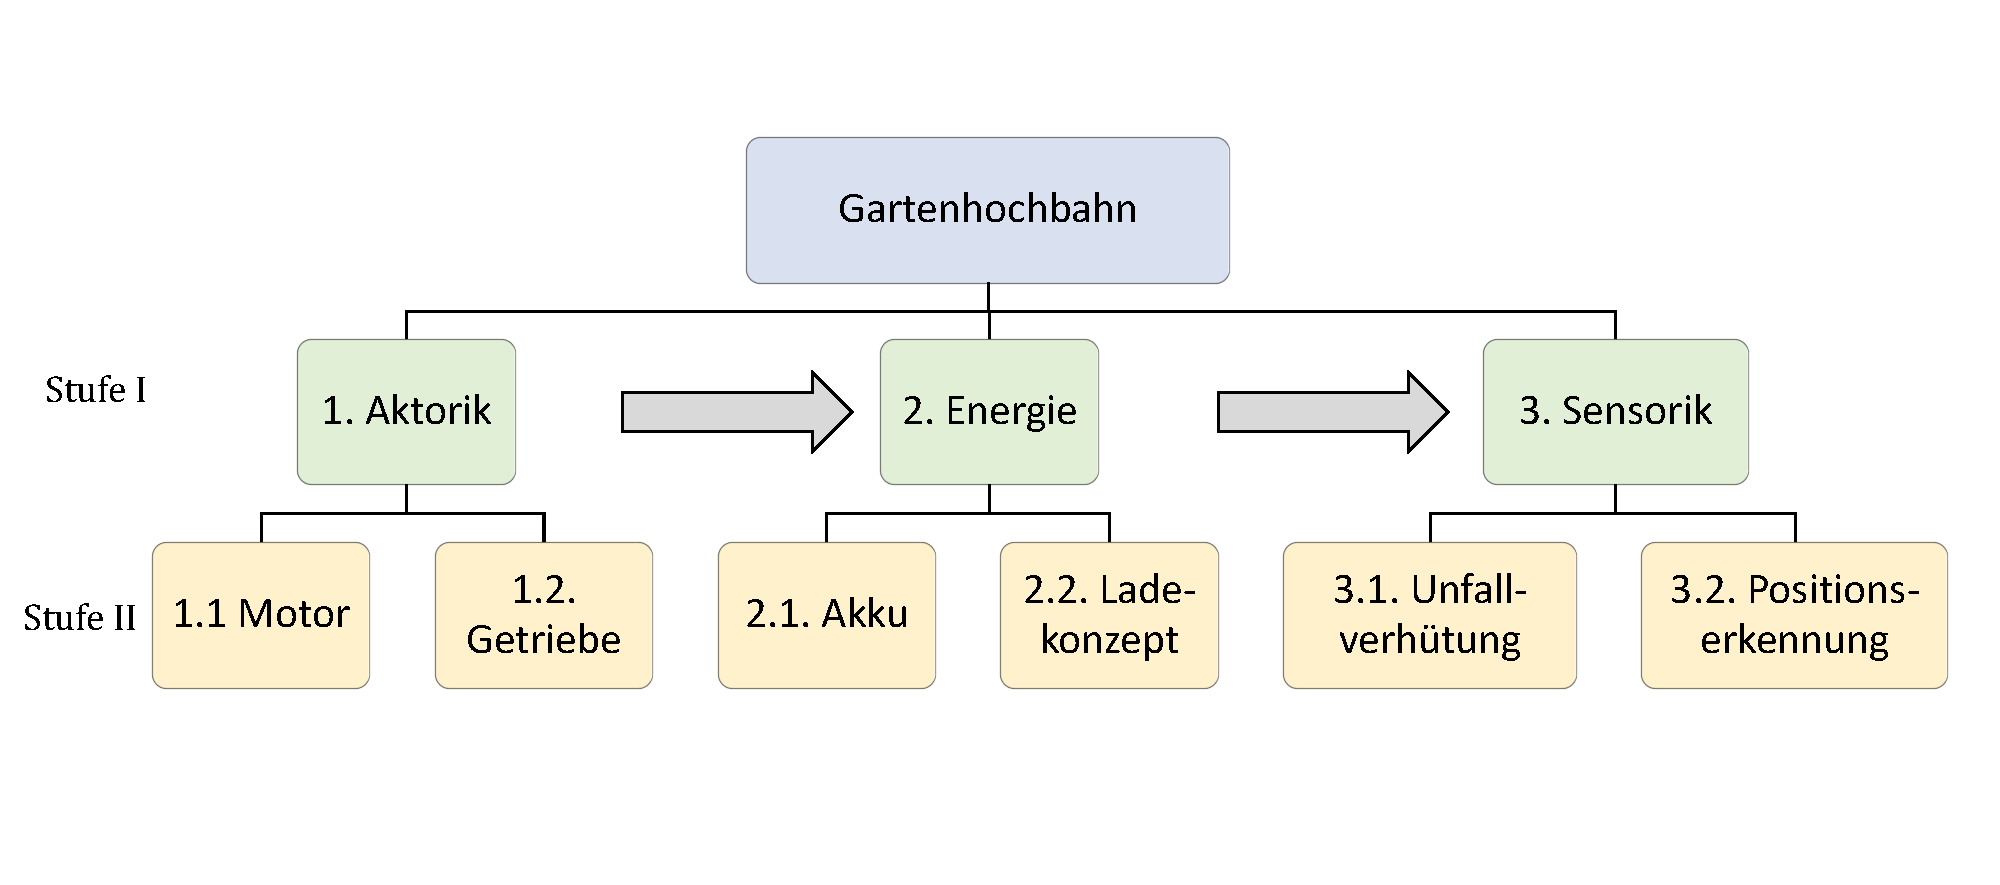
\includegraphics[width=17cm]{projektstrukturplan.pdf}
		\caption{Projektstrukturplan mechatronischer Komponenten}
		\label{pic:structuremech}
	\end{center}
\end{figure}

Das Projekt ist untergliedert in drei Teilaufgaben. Diese werden in der nächsten Ebene in Arbeitspakete untergliedert. 
Da die Bereiche aufeinander aufbauend sind, können Zusammenhänge analysiert werden. In dem Schaubild sind die Bereiche von links nach rechts in zeitlicher Abfolge aufgetragen. Dementsprechend soll in einem ersten Schritt die Aktorik konzeptioniert werden. Dazu zählt die elektrische und mechanische Komponente des Antriebs. Mit den elektrischen Leistungsdaten der Aktorik wird im nächsten Schritt das Energiekonzept ausgearbeitet. Auf diesen Bereich baut final die Konzeptionierungsphase der Sensorik auf. \\ 

\newpage
\subsection{Projektablaufplan}
\label{sec:projektablaufplan}
Aus dem Projektstrukturplan geht der Projektablaufplan hervor. Darin werden die zuvor definierten Arbeitspakete aus den Teilaufgaben terminiert. Ein Ausschnitt aus dem Projektablaufplan der mechatronischen Komponenten ist in \autoref{pic:roadmap} dargestellt. 
\begin{figure}[h]
	\begin{center}
		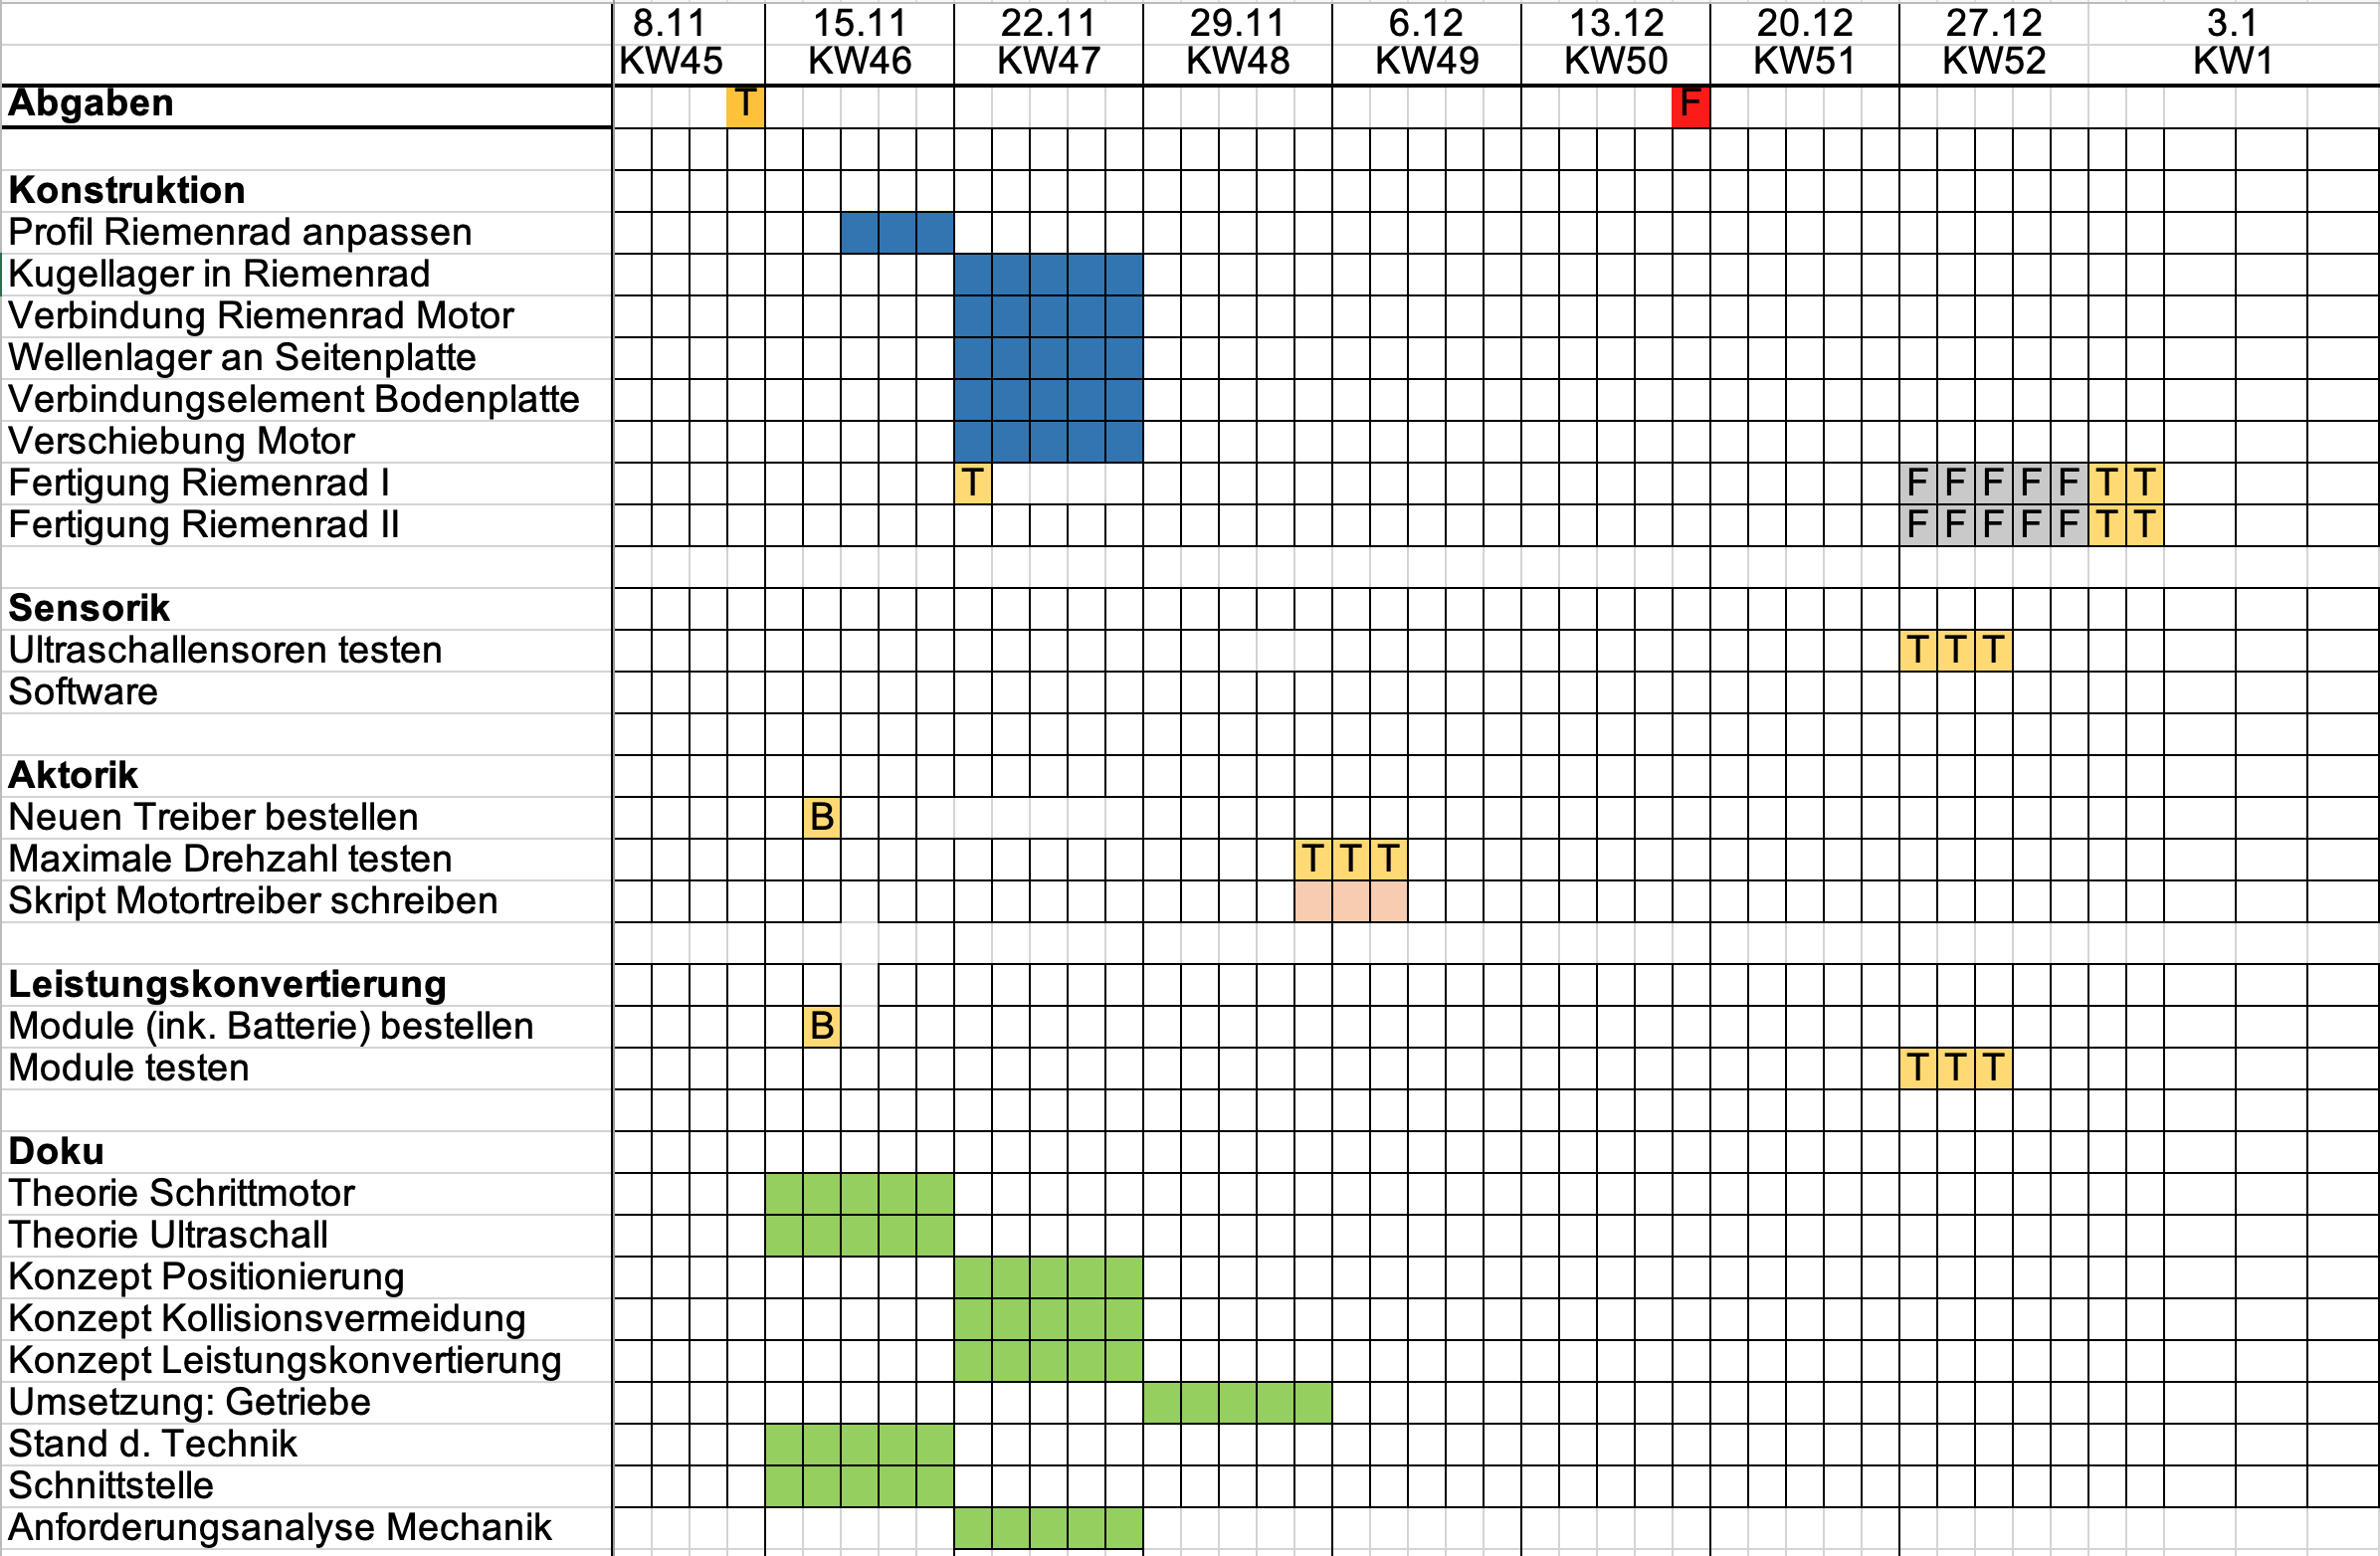
\includegraphics[width=17cm]{roadmap.png}
		\caption{Projektablaufplan mechatronischer Komponenten}
		\label{pic:roadmap}
	\end{center}
\end{figure}



\newpage
\subsection{Arbeitsmangement}
\label{sec:arbeitsmanagement}
Für das Arbeitsmanagement wird die Kanban-Methode verwendet. Dabei werden die Teilaufgaben dem Bearbeitungsstatus zugeordnet. Im Rahmen des Projektes wurden die Stati \textit{Backlog}, \textit{Todo,  In Progress, Testing} und \textit{Done}  unterschieden. 
Die Aufgaben wurden mit den Berbeitungszeiträume aus dem Projektablaufplan definiert und dem entsprechenden Bearbeiter zugewiesen. 	
Für die Kanban-Methode kam das Tool \textit{Trello} zum Einsatz. 


%----------------------KONZEPT-------------------------

\chapter{Konzeptionierung der mechatronischen Komponenten}
\label{cha:konzeptionierung}
Mit \autoref{cha:anforderungsanalyse} wurden Anforderungen an das Projekt gestellt. Zum Erreichen dieser Anforderungen findet in diesem Kapitel die Konzeptionierung statt. Dazu wird mit \autoref{sec:konzeptGrundaufbau} zunächst der generelle Aufbau betrachtet. Anschließend folgen mit den Abschnitten \ref{sec:konzeptAktorik} bis \ref{sec:konzeptSensorik} die Konzepte zu den mechatronischen Komponenten \textit{Aktorik}, \textit{Energieversorgung} und \textit{Sensorik}. Als Übergang zu den informationstechnischen Konzepten werden mit \autoref{sec:konzeptSchnittstellen} die \textit{Schnittstellen} ausgearbeitet. \newpage

\section{Grundaufbau}
\label{sec:konzeptGrundaufbau}
Beim Aufbau der neuen Gondel wird das grundlegende Prinzip des bisherigen Aufbaus übernommen. Dazu zählt, dass die Gondel mit zwei Elementen in die Schiene eingehängt wird. Die beiden Baugruppen werden nachfolgend als \textit{Triebwagen} und \textit{Stützwagen} bezeichnet. Beide Elemente besitzen ein Paar Laufrollen für die Fortbewegung auf der Schiene. Im Triebwagen sind zusätzlich Motor und Getriebe verbaut. An den beiden Baugruppen werden nach unten Verbindungselemente für die Befestigung des Tabletts sowie für die Elektronik angebracht. Zur besseren Veranschaulichung ist in  \autoref{pic:grundaufbau} die Konstruktion der beiden Wägen dargestellt. Die Beschreibung der Konstruktion folgt im Teil der \textit{Umsetzung} in \autoref{cha:umsetzung}.


\begin{figure}[h]
	\centering
	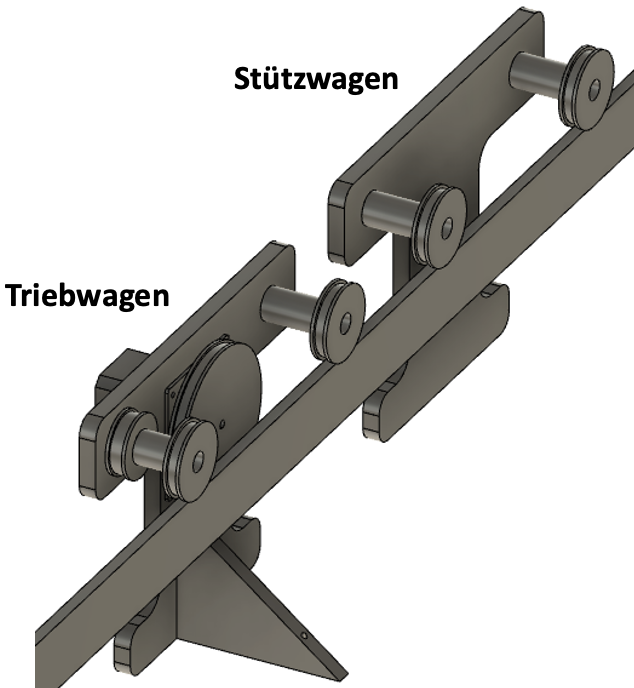
\includegraphics[width=8cm]{grundaufbau.png} 
	\caption{Konstruktionsansicht von Trieb- und Stützwagen}
	\label{pic:grundaufbau}
\end{figure}
Eine dringende Anforderung an den Aufbau ist, dass die Gondel stets lotrecht hängt. Aus diesem Grund wir nun das Kippmoment betrachtet. 
\newpage

\textbf{Ausgleich des Kippmoments}\\
 Durch die einseitige Belastung des Motors ergibt sich vor allem beim Triebwagen ein Kippmoment. Eine mögliche Lösung wäre, das Kippmoment durch eine Laufrolle auf der Seitenfläche der Schiene abzufangen. Aufgrund der Befestigung der Schiene ist dies jedoch nicht möglich. Aus diesem Grund soll das Kippmoment durch ein entgegengesetztes Drehmoment mit einem Gewicht erzeugt werden. In \autoref{pic:kippmoment} ist der Zusammenhang veranschaulicht. 

\begin{figure}[h]
	\centering
	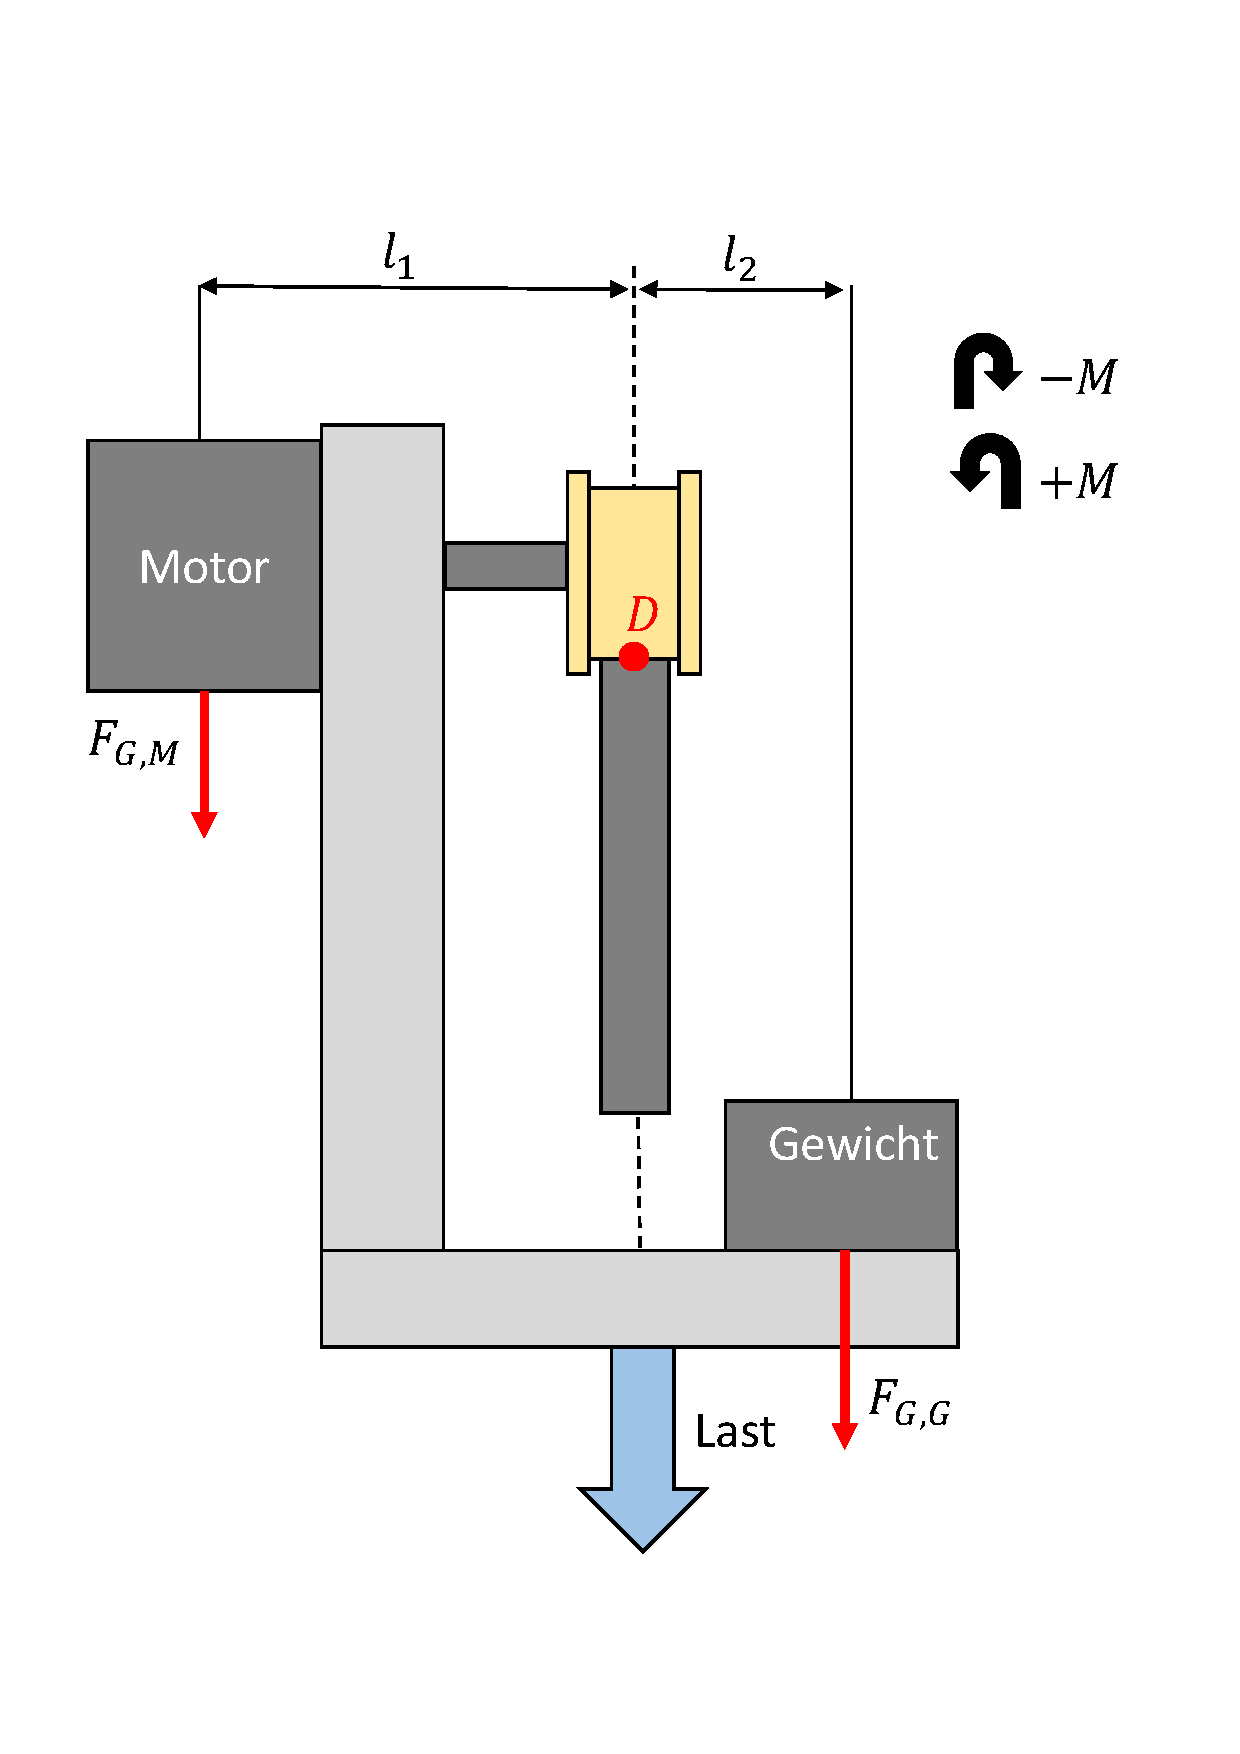
\includegraphics[width=10cm]{kippmoment.pdf} 
	\caption{Betrachtung des Kippmoments am Triebwagen}
	\label{pic:kippmoment}
\end{figure}
Der Aufbau dreht sich um den Punkt $D$. Für die lotrechte Ausrichtung der Gondel muss gelten, dass 

\begin{align}
	\sum M_D = 0
\end{align}
\newpage 

 Der Motor hat mit einer Masse von $300g$ eine Gewichtskraft von $F_{G,M} \approx 2,94N$. Der Hebelarm ist $l_1=70mm$. Dieses positive Drehmoment soll mit einem negativen Moment durch das Gewicht mit der Kraft $F_{G,G}$ und Hebelarm $l_2$ ausgeglichen werden. Bei gegebenem Hebelarm $l_2$ ergibt sich dabei für die erforderliche Masse des Gewichtes:

\begin{align}
	m_G = m_M \cdot \frac{l_1}{l_2}
\end{align}
 
In der Praxis gilt es zu untersuchen, inwiefern ein zusätzliches Gewicht beim Stützwagen notwendig ist. Generell ist anzunehmen, dass durch die Last des Tablets die Gondel zusätzlich stabilisiert wird.  

\section{Aktorik}
\label{sec:konzeptAktorik}
In diesem Abschnitt wird die Konzeptionierung des Antriebs der Gartenhochbahn beschrieben. In \autoref{sec:konzeptMotor} wird zunächst die Auswahl und Auslegung des Motors erläutert. Das Drehmoment des Motors soll anschließend auf ein Laufrad übertragen werden. Die Beschreibung des dafür zuständigen Getriebes folgt mit \autoref{sec:getriebekonzept}

\subsection{Motor}
\label{sec:konzeptMotor}
Für den Antrieb der Gartenhochbahn wurde zwischen einem DC-Motor und einem Schrittmotor ausgewählt. Bei einem DC-Motor wird ein \acrshort{pwm}-Signal angelegt. Dieses wird von einem Treiber generiert. Bei einem Schrittmotor werden bei der Steuerung von einem Treiber positive Taktflanken des Controllers ausgewertet. Wie in \autoref{sec:schrittmotor} beschrieben, werden je nach Betriebsmodus pro Taktflanke die Spulen des Motors entsprechend bestromt. Durch den Zusammenhang zwischen Taktflanken und  Inkrementalschritten des Motors können Rückschlüsse auf die zurückgelegte Strecke gemacht werden.  

Da die Information der Wegstrecke für die Positionsbestimmung genutzt werden kann, soll für die Gartenhochbahn ein Schrittmotor verwendet werden. Dafür kommt der Hybrid-Schrittmotor Nema 17-04 von Joy-IT zum Einsatz. Als Schrittmotortreiber wird der DRV8834 von Texas Instruments verwendet. 


\subsection{Getriebe}
\label{sec:getriebekonzept}
Das Getriebe sorgt für die Kraftübertragung des Motordrehmoments auf die Schiene. Zusätzlich ist die Geschwindigkeit der Hochbahn vom Übersetzungsverhältnis des Getriebes abhängig. Nachfolgend wird die Auswahl der Getriebeart und anschließend die Auslegung beschrieben. \\

\textbf{Getriebeart}\\
Für die Auswahl der Getriebe steht ein Zahnradgetriebe und ein Zugmittelgetriebe im Raum. Das Zahnradgetriebe besitzt eine formschlüssige Kraftübertragung der beiden Räder. Damit diese mit dem geeigneten Kopfspiel zustande kommt, müssen die beiden Wellen in einem exakten Abstand zueinander stehen. Das bedarf einem hohen Grad an Präzision bei der Fertigung. Bei einem Zugmittelgetriebe kann bspw. eine Spannrolle dafür sorgen, dass das Zugmittel ausreichend gespannt ist. Dadurch muss der Abstand der beiden Räder zueinander ein niedrigeres Maß an Genauigkeit besitzen. 
Für das Projekt wird ein Zugmittelgetriebe verwendet. Um dabei Schlupf zu vermeiden, wird ein T-Profil bei Riemen und Rad verwendet. 
\\

\textbf{Konstruktion und Fertigung}\\
Der Antrieb besteht aus den folgenden Komponenten: \textit{getriebenes}- und \textit{treibendes Riemenrad, Laufrad} und \textit{Zahnriemen}. Zunächst wird das Konzept für das getriebene Riemenrad und das Laufrad beschrieben. Anschließend erfolgt die Beschreibung des gesamten Antriebs anhand der Konstruktion.  
Das Laufrad kommt für den Abtrieb auf der Schiene zum Einsatz. Eine Herausforderung stellt dabei die Kraftübertragung vom Laufrad auf das getriebene Riemenrade dar. Dazu wurden zwei Konzept entwickelt. Die Gegenüberstellung ist in \autoref{pic:abtriebkonzepte} dargestellt.
\newpage

\begin{figure}[h]
	\begin{center}
		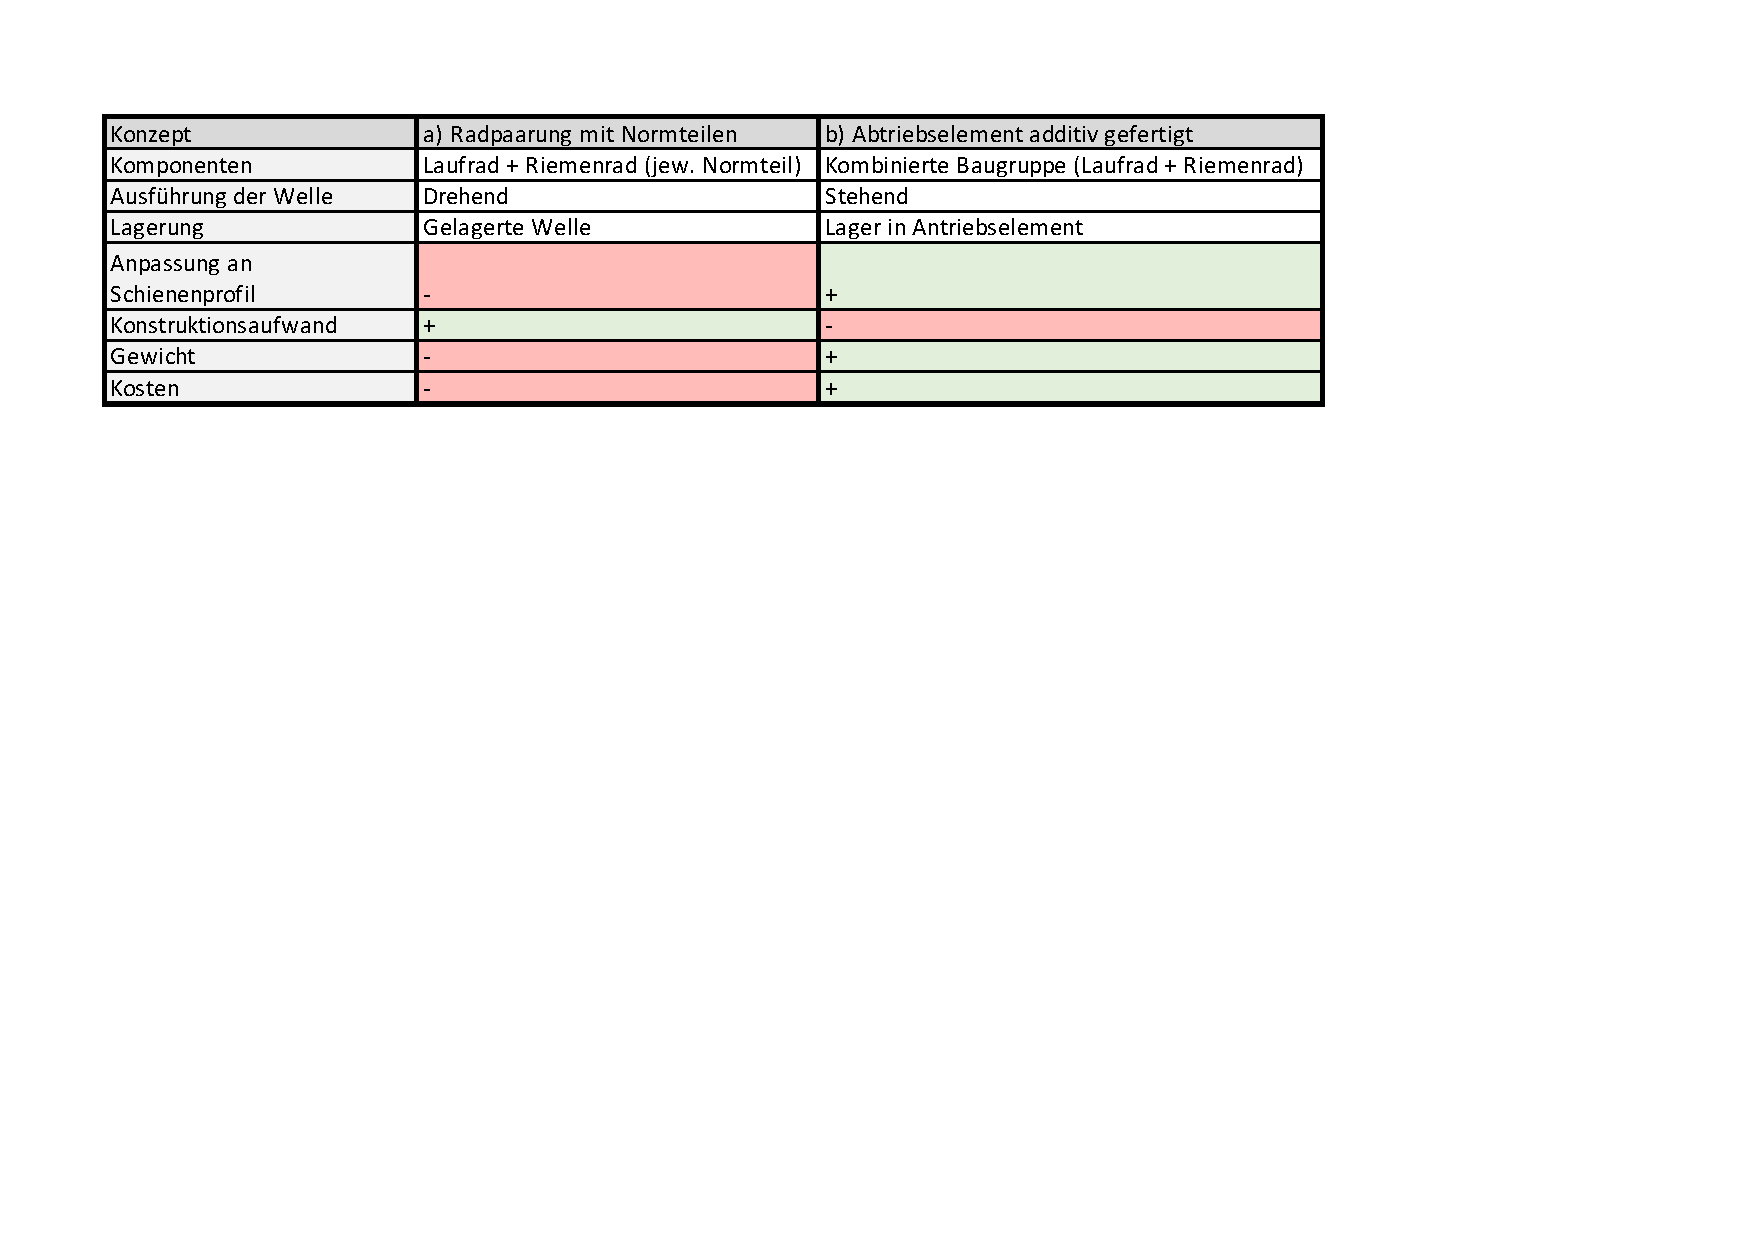
\includegraphics[width=17cm]{abtriebkonzepte.pdf}
		\caption{Konzepte für die Kraftübertragung vom Riemenrad auf das Laufrad}
		\label{pic:abtriebkonzepte}
	\end{center}
\end{figure}


Bei Konzept a) wird für Lauf- und Riemenrad jeweils ein Normteil verwendet. Die Kraftübertragung zwischen den beiden Rädern erfolgt über eine Welle. Diese ist gelagert, während die beiden Räder stehend auf der Welle montiert sind. Die Normteile der beiden Räder sind meist für hohe Krafteinwirkungen in industriellem Einsatz ausgelegt. Dadurch ergibt sich bei Verwendung der Räder ein hohes Gewicht. Die Bauteile sind jedoch mit hohen Kosten verbunden.

Bei Konzept b) sind Laufrad und Riemenrad eine Baugruppe. Das kombinierte Bauteil wird additiv gefertigt und ist stehend auf der Welle gelagert. Die Welle selbst ist ebenfalls stehend ausgeführt. Durch die additive Fertigung ist eine CAD-Konstruktion zwingend notwendig. Dadurch ergibt sich in diesem Punkt ein höherer Aufwand als bei der Verwendung von Normteilen. Die Konstruktion bietet jedoch den Vorteil, dass das Laufrad an das Profil der Schiene angepasst werden kann. 

Für das Projekt wird Konzept b) verfolgt. Die additive Fertigung des Bauteils sollte für die Krafteinwirkung ausreichend sein und die Kosten können somit geringer gehalten werden. 

\newpage

\section{Energieversorgung}
\label{sec:konzeptEnergieversorgung}
Die Batterie dient als Energieversorgung für Aktorik, Sensorik und Steuerung. Um für die Komponenten passende Ströme und Spannungen bereitstellen zu können, ist eine Leistungskonvertierung notwendig. In \autoref{pic:leistungskonvertierung} sind die zu diesem Zweck verwendeten Komponenten dargestellt und in \autoref{tbl:leistungskonvertierung} aufgelistet. 

\begin{figure}[h]
	\begin{center}
		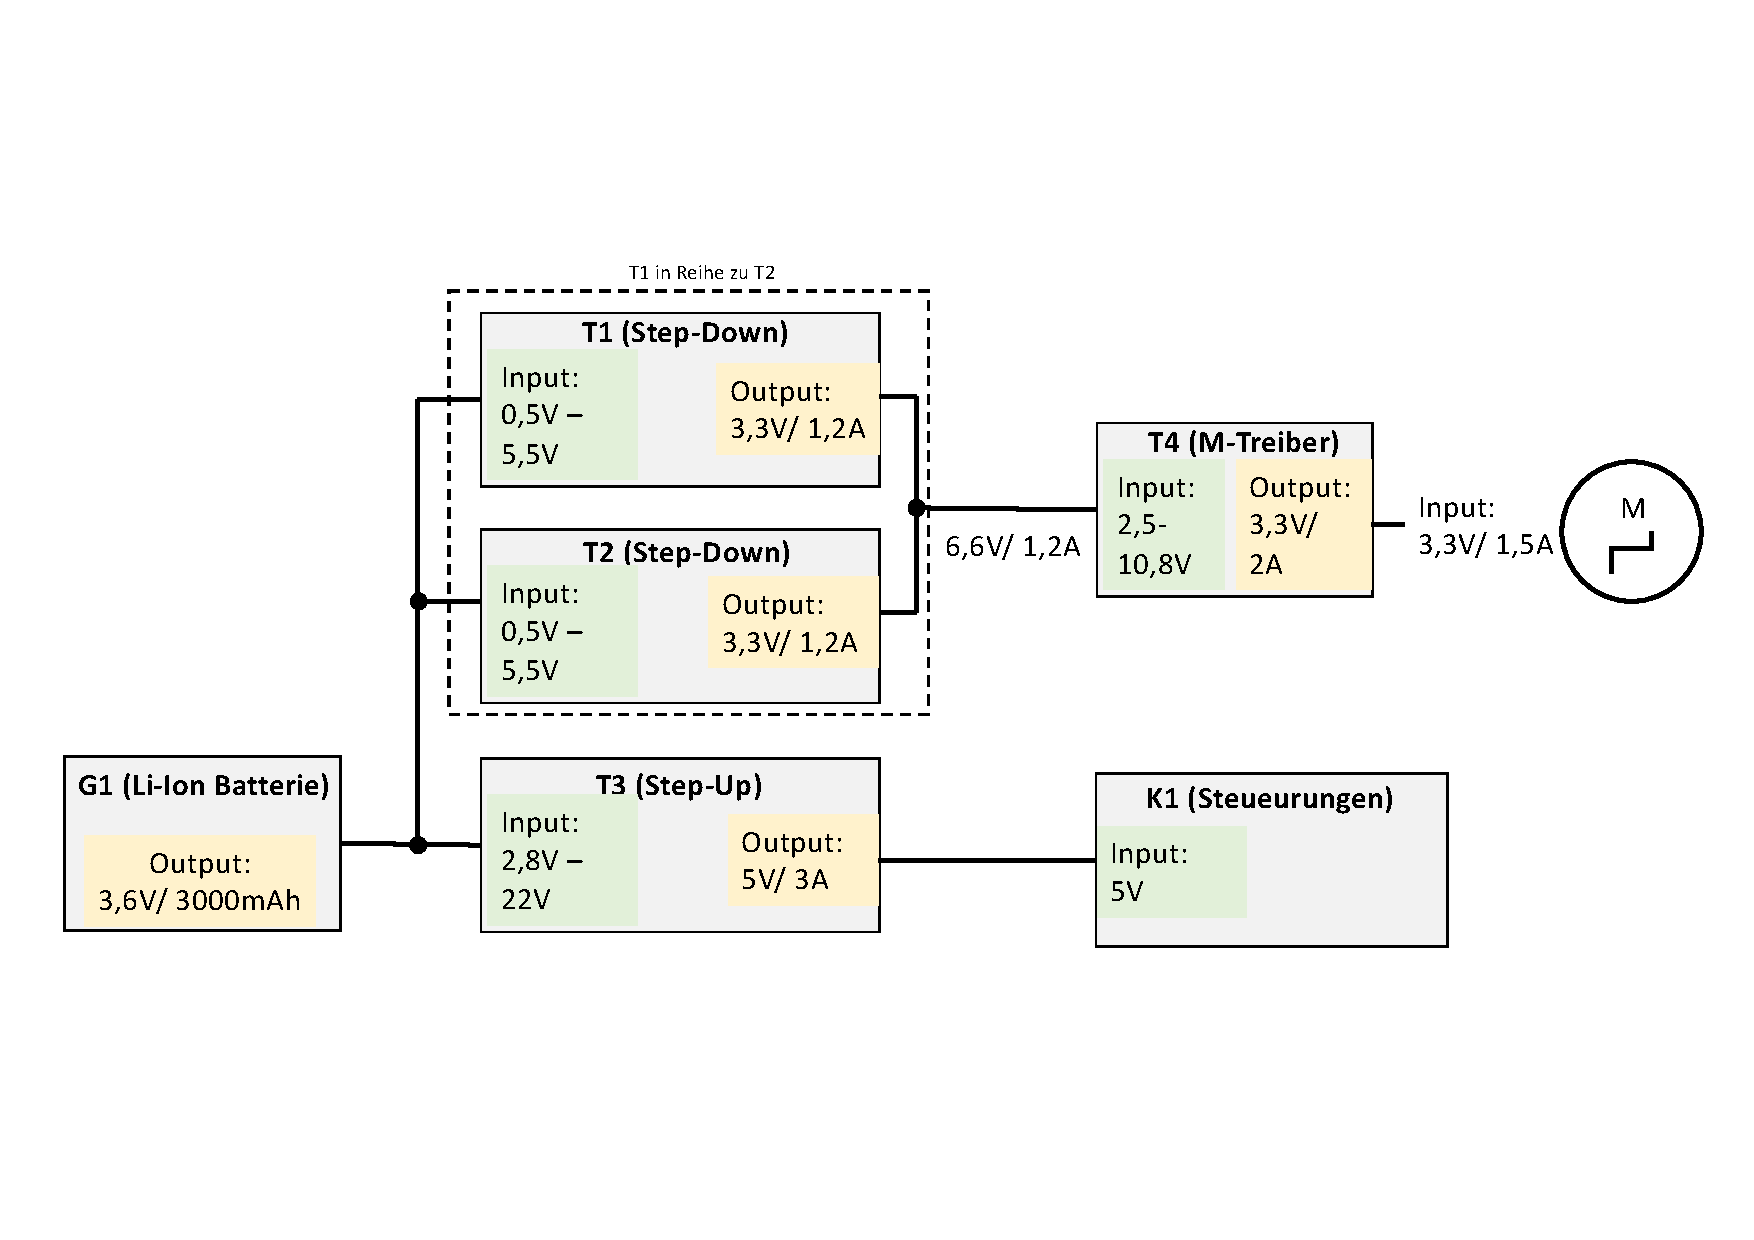
\includegraphics[width=17cm]{leistungskonvertierung.pdf}
		\caption{Schema zur Leistungskonvertierung der elektrischen Komponenten}
		\label{pic:leistungskonvertierung}
	\end{center}
\end{figure}


\begin{table}[h]
	\begin{center}
		\begin{tabular}[h]{l|l|l}
			\textbf{Name} & \textbf{Bezeichnung} & \textbf{Bauteill}\\
			\hline
			G1 & Li-Ion Batterie & Panasonic NCR18650B\\
			\hline
			T1-T2 & Step-Down Converter & Polulu S13V30F5\\
			\hline
			T3 & Step-Up Converter & Polulu U1V11F3\\
			\hline
			T4 & Schrittmotor Treiber & Polulu DRV8834 \\
			\hline
			K1 & Steueurungen & Arduino Nano, ESP32 \\
		\end{tabular}
	\end{center}
	\caption{Bezeichnungen verwendeter Komponenten}
	\label{tbl:leistungskonvertierung}
\end{table}
\newpage

Die Li-Ion Batterie darf eine minimale Zellspannung $U_{min} =2,75V$ nicht unterschreiten. Zu diesem Zweck lässt sich die \acrshort{cutoffvoltage} bei den beiden Step-Down Convertern $T1$ und $T2$ einstellen. Damit wird bei  niedrigem Batteriezustand die Leistungselektronik abgeschaltet. Die Steuerung ist anschließend noch immer aktiv, sodass eine Kommunikation mit dem Hochbahncontroller weiterhin möglich bleibt. Im Schema nicht dargestellt ist der Hochbahncontroller ESP32, der die Entladespannung ebenfalls kontinuierlich überprüft und vor Erreichen der \acrshort{cutoffvoltage} die Fahrt zur Ladestation einleitet. Die beiden Konverter $T1$ und $T2$ sind in Reihe geschaltet, um die erforderlichen Leistungen des Schrittmotors bereitstellen zu können. Am Schrittmotortreiber $T4$ lässt sich die für den Motor geforderte Spannung und maximale Stromstärke einstellen. Dafür findet im Treiber ebenfalls eine Leistungskonvertierung von $V_{in}=6,6V$ auf $V_{Motor}=3,3V$ statt. Der Step-Up Converter $T3$ passt die Eingangsspannung an die erforderliche Spannung der Controller an. Die Ausgangsspannung des Converters liegt bei $5 \pm 0,15 V$ \\

Die Li-Ion Batterie soll in der Parkposition der Hochbahn aufgeladen werden. Die Batterie kann bei einer Ladespannung von $4,2V$ aufgeladen werden. Für die Steuerung des Ladevorgangs kommt der Ladecontroller $MCP73831/2$ von Microchip zum Einsatz. Der Controller lässt einen Ladestrom von $500mA$ zu. 


\newpage

\section{Sensorik}
\label{sec:konzeptSensorik}
Zur $Kollisionsvermeidung$ und $Positionserfassung$ kommen Sensoren zum Einsatz. Diese werden in den nächsten beiden Abschnitten beschrieben.

\subsection{Kollisionsvermeidung}
\label{sec:konzeptKollisionsvermeidung}
Für die Kollisionsvermeidung soll mithilfe von Ultraschallsensoren kontinuierlich die Distanz $d$ zum nächsten Objekt gemessen werden. Als Sensoren werden zwei HC-SR04 auf dem Tablett angebracht. Der Messbereich beträgt $0,02m - 5m$ (\cite{hcrs04}). Der Sensorbereich soll in ein Warn- und Schutzfeld eingeteilt werden. Das Warnfeld wird verletzt, wenn bei mindestens einem der beiden Sensoren $d<1,5m$ erfüllt ist. Eine Schutzfeldverletzung erfolgt bei $d<0,7m$. 

In \autoref{pic:kollisionsvermeidung} sind die beiden Ultraschallsensoren mit Warn- und Schutzfeld dargestellt. 

\begin{figure}[h]
	\begin{center}
		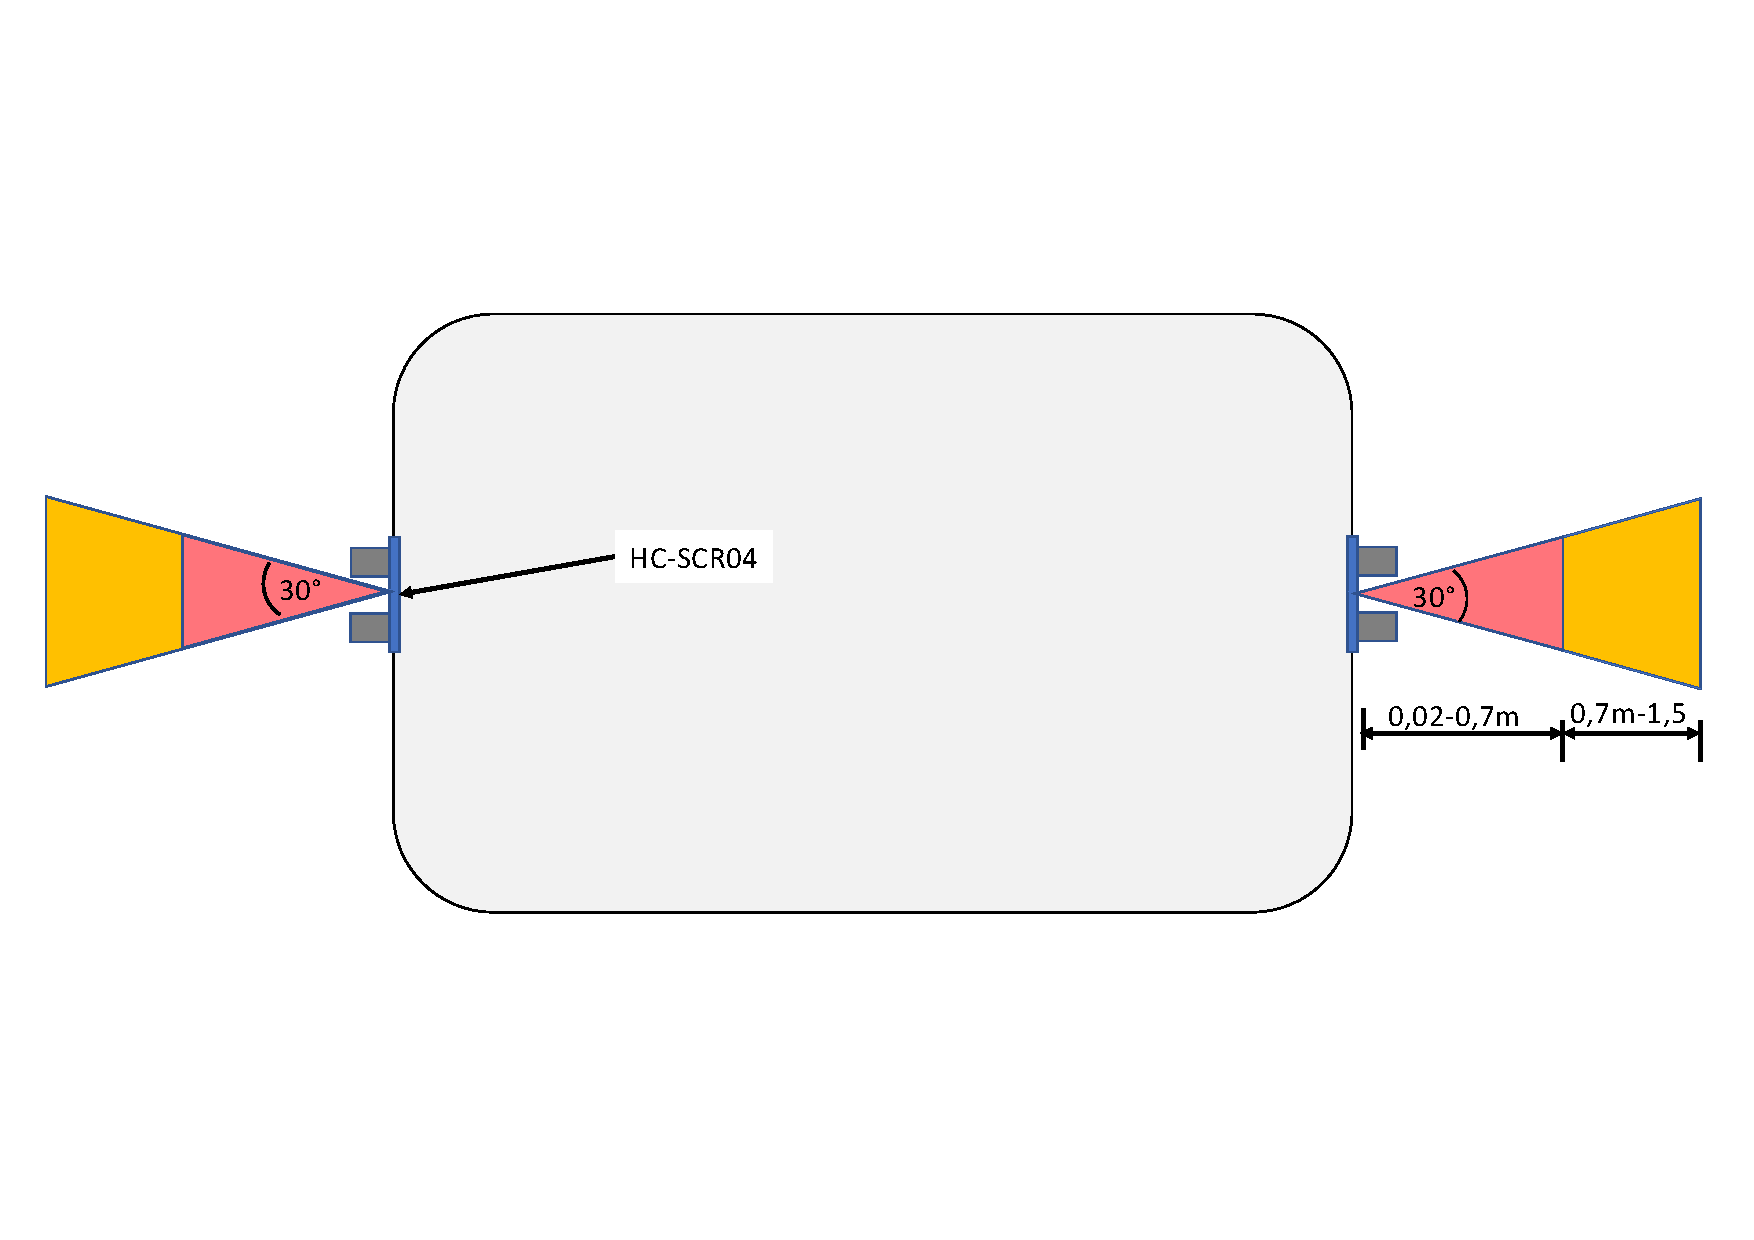
\includegraphics[width=16cm]{kollisionsvermeidung.pdf}
		\caption{Schematische Anordnung der Ultraschallsensoren HC-SR04 auf dem Tablett zur Kollisionsvermeidung mit den Warn- und Schutzfeldbereichen}
		\label{pic:kollisionsvermeidung}
	\end{center}
\end{figure}
\newpage

Die Breite $b$ des kleinsten zu erfassende Objektes beim Öffnungswinkel $\alpha = 30^{\circ}$ beträgt:

\begin{align}
	b= tan(\alpha) \cdot d \cdot 2
\end{align}

 Dabei beträgt das kleinste erfassbare Objekt am Ende des Schutzfelds $b_S \approx 0,4m$ und am Ende des Warnfelds $b_W \approx 0,8m$. \\
 
Der Ultraschallsensor HC-SCR04 Ultraschallsensor verfügt für die Messung der Schalllaufzeit über die beiden Pins \textit{TRIG} und \textit{ECHO}. Die Messung wird durch eine fallende Flanke von 10µs am Triggereingang gestartet. Anschließend werden über den  Piezokristall des Sensors acht aufeinanderfolgende 40Khz Schallwellen ausgesandt. Nach 200µs setzt der Sensor \textit{ECHO} so lange auf high, bis der Ultraschallimpuls empfangen wurde. Wurde keine Schallreflektion empfangen, verbleibt  \textit{Echo} für max. 38 ms auf HIGH. Eine erneute Messung kann frühestens nach 20ms gestartet werden. (vgl. \cite{hcrs04})

Mit einem Arduino Nano werden die Messungen an beiden Sensoren zyklisch durchgeführt. Die Berechnung der Distanz erfolgt anhand der in \autoref{sec:ultraschall} beschriebenen Formel. Tritt eine Schutz- oder Warnfeldverletzung auf, gibt der Arduino ein Signal auf einen entsprechenden Interrupt-Pin am ESP32 als  Hochbahn-Controller. Die verwendeten Interrupt-Pins sind nachfolgend dargestellt. \\


\begin{center}
	\begin{tabular}[h]{l|l|l}
		Sensor & Verletzung  & ESP32 Interrupt-Pin \\
		\hline
		1 & Warnfeld & GPIO1\\
		\hline
		1 & Schutzfeld & GPIO2\\
		\hline
		2 & Warnfeld & GPIO3\\
		\hline
		2 & Schutzfeld & GPIO4\\	
	\end{tabular}
\end{center}
\newpage

\subsection{Positionserfassung}
\label{konzeptPositionserfassung}
Die Position der Hochbahn entlang der Strecke soll kontinuierlich erfasst werden. Dafür kommen zwei Lokalisierungsmethoden zum Einsatz: 

 \begin{itemize}
 	\item [a)] Absolute Positionserfassung durch einen \acrshort{reed}-Kontakt
 	\item[b)] \acrshort{lagekopplung} auf Basis des Feedbacks der Motorsteuerung  
 \end{itemize}

Für die absolute Positionserfassung sollen entlang der Strecke Dauermagneten in einem Abstand von 1,5m angebracht werden. Die Magneten schließen den Kontakt des  \acrshort{reed}-Schalters auf der Hochbahn. Zusammen mit der Information zur Fahrtrichtung wird ein Zählwert auf dem Hochbahncontroller ESP32 inkrementiert bzw. dekrementiert. Auf Basis des Feedbacks der Motorsteuerung wird aus der aktuellen Geschwindigkeit die diskrete Position zwischen den Magneten berechnet. Diese Art der \acrshort{lagekopplung} ist prinzipbedingt fehlerbehaftet. Daher wird bei absoluten Markern der Inkrementalwert zurückgesetzt. 
\newpage

\section{Schnittstellen}
\label{sec:konzeptSchnittstellen}
Als Übergang von der Konzeptionierung mechatronischer Komponenten zu den informationstechnischen Konzepten soll in diesem Abschnitt die Schnittstelle aller verwendeten Komponenten vorgestellt werden. Dazu ist in \autoref{pic:schnittstellen} eine Übersicht dargestellt.

\begin{figure}[h]
	\centering
	\includegraphics[width=16cm]{schnittstellen.pdf}
	\caption{Schnittstellenübersicht der verwendeteter Komponenten}
	\label{pic:schnittstellen}
\end{figure}

In dem Schema sind die Komponenten hierarchisch dargestellt. Die Pfeile dazwischen stellen die Schnittstellen dar. Der Webserver kommuniziert mit den Endgeräten der Kunden oder dem Tablet in der Küche über \acrshort{http}. Mit POST-Requests werden Steuerbefehle oder Bestellungen zur weiteren Verarbeitung an den Server geschickt.
\acrshort{mqtt} dient zur Kommunikation zwischen dem Server und der Hochbahn. Für die Übermittlung der \acrshort{mqtt}-Befehle  befindet sich ein \acrshort{mqtt}-Broker auf der Kommunikationsebene. Die Hochbahn erhält Information über die Station, die angefahren werden soll. Während der Fahrt gibt die Bahn Rückmeldung über die aktuelle Position. Außerdem sollen Meldungen des Systems zur Kollisionsvermeidung und der Entladespannung der Batterie übertragen werden. Auf der Hochbahn führt ein ESP32 als Controller die Kommunikation durch. Die Steuerung des Motors und die Kollisionsvermeidung sind auf zwei Arduino Nanos ausgelagert. Der ESP32 ist den beiden Controllern übergeordnet. Für die Kommunikation zwischen der Motorsteuerung und dem ESP32 wird \acrshort{uart} zur seriellen Kommunikation verwendet. Der Hochbahncontroller versendet darüber Befehle zur Motorfrequenz und empfängt dafür von der Motorsteuerung die aktuelle Geschwindigkeit. \autoref{sec:motorsteuerung} beschreibt die Umsetzung der Motorsteuerung. Wie in Abschnitt \ref{sec:konzeptKollisionsvermeidung} beschrieben, überprüft die Sicherheitssteuerung kontinuierlich die Distanzwerte der Ultraschallsensoren. Ist eine Kollision zu erwarten, setzt die Steuerung einen entsprechenden Interrupt am Hochbahn-Controller. Der \acrshort{reed}-Kontakt für die Positionserfassung ist über $I/O$-Pins direkt mit dem Hochbahncontroller verbunden. 

\chapter{Entwicklung der Platine}
\label{sec:ecardConcept}
In \autoref{sec:konzeptSchnittstellen} wurde bereits angedeutet, dass auf der Hochbahn mehrere elektronische Komponenten zusammenarbeiten müssen (Arduino, ESP32, etc.). Daher werden diese Komponenten, sowie benötigte Peripherie, auf einer Platine zu einem verteilten System vereint. 
Die Entwicklung dieser Platine wird in Folgendem erläutert.

\section{Anforderungen an die Platine}
Folgende Anforderungen an die Platine müssen erfüllt sein: 
\begin{center}
	\begin{itemize}
		\item Kommunikation zwischen ESP32 und Arduino,
		\item Spannungsversorgung der einzelnen Mikrokontroller,
		\item Spannungsüberwachung beider Batteriezellen,
		\item Interruptleitungen von Reed-Kontakt und Kollisionsvorbeugung,
		\item Selbstabschaltung des Systems
		\item und Anschluss des Motortreibers.
	\end{itemize}
\end{center}
All diese Anforderungen sollen möglichst gering im Leistungsverbrauch sein. Das bedeutet, dass beispielsweise Spannungsteiler für die Spannungsüberwachung nur dann in Aktion treten, wenn auch wirklich Spannung gemessen wird. Ansonsten würde hierbei ein ständiger Stromverbrauch bestehen.

\section{Kommunikation zwischen ESP32 und Arduino}
Generell erfolgt die Kommunikation der beiden Mikrocontroller über \acrshort{uart}. Daraus folgt, dass \acrfull{rx}-Pin vom ESP32 mit \acrfull{tx}-Pin des Arduinos, sowie \acrshort{rx} des Arduinos mit \acrshort{tx} des ESP32 verbunden sein muss. 
Daraus resultiert folgendes Problem: der Arduino läuft mit einer Betriebsspannung von 5V, während der ESP32 mit 3,3V fungiert. Dadurch erhielte der ESP32 beim Empfangen von Nachrichten einen zu hohen HIGH-Pegel, während der Arduino Nachrichten mit zu niedriger Spannung bekäme.

\subsection{Level-Shifter}
Um die Pulse des ESP32 auf die richtige Spannung zu erhöhen, wird ein sogenannter Level-Shifter verwendet. Dieser übermittelt Signale mit einer Höhe von 5V an den Arduino, während der ESP32 nur 3,3V ausgibt.
Der zugehörige Schaltplan ist in \autoref{pic:levelshift} gezeigt.
\vspace{1cm}

\begin{figure}[h]
	\begin{center}
		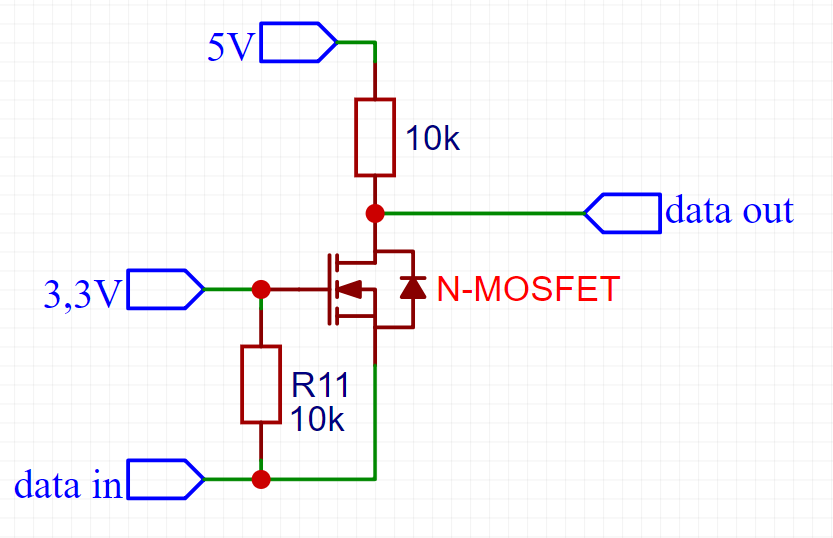
\includegraphics[width=9cm]{levelShifter.PNG}
		\caption{\label{pic:levelshift}Schaltplan des Level-Shifters}
	\end{center}
\end{figure}

Angenommen der ESP32 gibt an \textit{data in} ein \texttt{Low}-Signal, also 0V. Aufgrund der 3,3V am Gate des Mosfets schaltet sich dieses ein. Somit wird \textit{data out} durch das Mosfet ebenfalls auf 0V gezogen. 
Liegt \textit{data in} jedoch auf 3,3V, gibt es keinen Spannungsunterschied zwischen Gate und Source des Mosfets. Dies deaktiviert das Mosfet, sodass \textit{data out} auf 5V gezogen wird. 
Somit erzeugt eine positive Flanke von 3,3V des ESP32 eine Flanke von 5V am Arduino.

\subsection{Spannungsteiler}
Um 5V Pulse auf 3,3V zu ziehen, ist nicht zwingend eine Mosfet oder Transistorschaltung nötig. Hierbei genügt ein Spannungsteiler. Dieser ist in \autoref{pic:spannungsteiler} gezeigt.

\begin{figure}[h]
	\begin{center}
		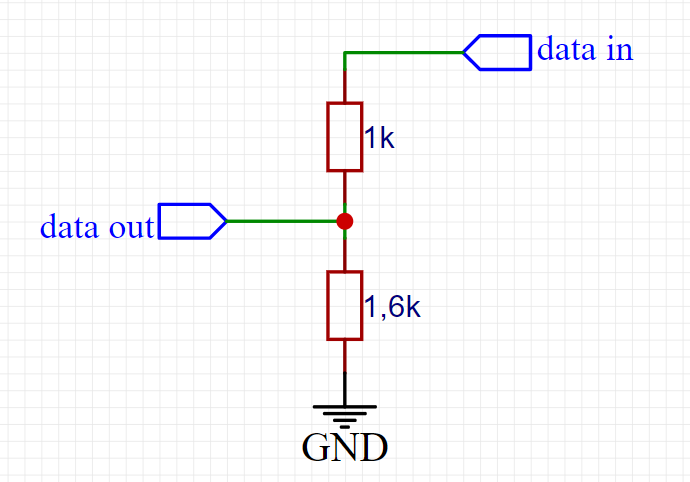
\includegraphics[width=9cm]{spannungsteiler.PNG}
		\caption{\label{pic:spannungsteiler} Spannungsteiler zur Kommunikation von Arduino zu ESP32}
	\end{center}
\end{figure}

Aus dem Verhältnis von $1 \div 1,6$ der beiden Widerstandsgrößen wird eine Ausgansspannung von ca. 3,08V bei einem 5V Pegel erzeugt. Diese wird in jedem Fall als logisches \texttt{High} interpretiert.

\subsection{Spannungsversorgung}
Auf der Platine gibt es drei unterschiedliche Betriebsspannungen: 
\begin{center}
	\begin{itemize}
		\item 3,3V für den ESP32,
		\item 5V für beide Arduini und Stepper-Driver
		\item und 10V für den Schrittmotor.
	\end{itemize}
\end{center}
All diese Spannungen kommen aus der Stromquelle, welche aus den zwei Zellen des Litium-Ionen Akkus besteht. Die Spannung liegt je nach Ladezustand zwischen ca. 7,4V und 8,2V. Da die Komponenten jedoch zu jedem Zeitpunkt die gleiche Spannung benötigen, werden Spannungsregler benötigt. 
Einer davon ist ein DCDC-Wandler, welcher die Zellspannung auf konsistente 5V für die Arduini regelt. Da der ESP32 besitzt selbst einen Spannungsregler von 5V auf 3,3V besitzt, kann dieser ebenfalls an die Arduino-Versorgungsleitung gelegt werden. Wie schon in TODO erwähnt, erzeugt ein Step-Up-Wandler eine Spannung von 10V für Motortreiber und Schrittmotor. 

\section{Spannungsmessungen an den Batteriezellen}
\label{sec:mess}
Die Stromversorgung der Hochbahn stellen zwei in Reihe geschaltete Lithium Ionen Akkus zur Verfügung. Diese Reihenschaltung ist in \autoref{pic:messfalsch} gezeigt. Während bei einfachen Batterien die Gesamtspannung gemessen werden kann, müssen hier die beiden Zellen einzeln betrachtet werden.
Um die einzelnen Zellen zu messen, soll die Spannung jeweils am + Pol abgegriffen werden. Somit muss die Messeinrichtung von der Gesamtspannung jene der ersten Zelle abziehen, um die Spannung der zweiten Zelle zu erhalten. Dieser Vorgang ist erforderlich, da kein Spannungsunterschied zwischen + und - der oberen Zelle gemessen werden kann. Grund dafür ist, dass \gls{gnd} des Arduinos gleich mit \gls{gnd} der unteren Zelle ist, nicht der oberen.
\newpage Verbände man, wie in \autoref{pic:messfalsch} gezeigt, zwei analoge Pins direkt mit den + Polen, wäre eine Spannungsmessung in der Theorie möglich.

\begin{figure}[h]
	\begin{center}
		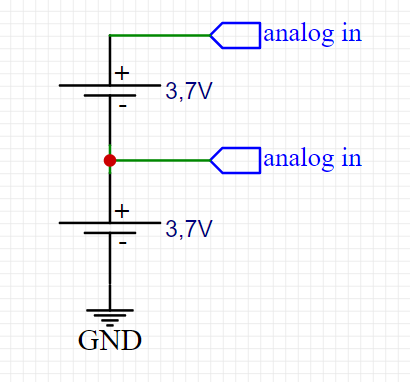
\includegraphics[width=8cm]{wrongMeasure.PNG}
		\caption{\label{pic:messfalsch} Einfache Spannungsmessung der Zellen}
	\end{center}
\end{figure}

In der Praxis ergeben sich dabei jedoch zwei Probleme:

\begin{center}
	\begin{itemize}
		\item 1. Wenn die Spannungsversorgung der Platine abgeschaltet ist, würde ein Arduino sich über die analogen Pins selbst versorgen, wodurch ein unnötiger Stromverbrauch entstände. Dadurch würden sich die beiden Zellen im Schlimmsten Fall tiefenentladen.
		\item 2. Ein Arduino kann nur Spannungen zwischen 0V und 5V messen, wodurch eine Reihenschaltung der beiden 3,7V Zellen auch im entladenen Zustand am analogen Input 5V, also 100\%, erzeugen. 
	\end{itemize}
\end{center}

Die im folgenden erklärte Schaltung soll diese Probleme umgehen.
\newpage
\subsection{Mosfetschaltung zur aktivierbaren Spannungsmessung}
Diese Schaltung soll ermöglichen, die Spannungsmessung per Signal aktivieren zu können. Das Signal wird dabei vom messenden Arduino mit einem 5V-Pegel erzeugt. Aktiviert, sollen ähnlich wie in \autoref{pic:messfalsch} beide Spannungen abgegriffen werden.

\begin{figure}[h]
	\begin{center}
		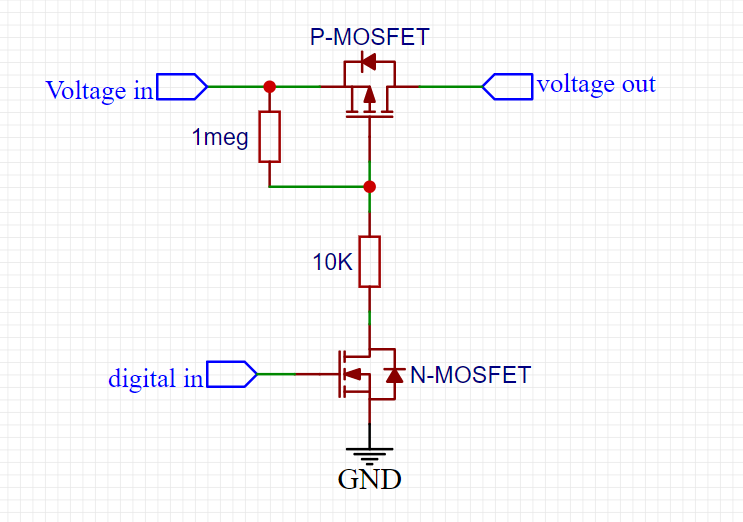
\includegraphics[width=11cm]{messRichtig.PNG}
		\caption{\label{pic:messrichtig} Mosfetschaltung zur aktivierbaren Spannungsmessung}
	\end{center}
\end{figure}

Die Mosfetschaltung zur Messung der ersten unten liegenden Zelle ist in \autoref{pic:messrichtig} gezeigt.
Zu sehen sind ein p- und ein n-Kanal Mosfet. Das unten geschaltete n-Kanal-Mosfet verbindet bei einer positiven Spannung auf \textit{digital in} das Gate vom p-Kanal-Mosfet mit \gls{gnd}. Dadurch wird das p-Kanal-Mosfet geschaltet, wodurch bei \textit{voltage out} eine Spannungsmessung möglich wird. Die Spannung ist jene, die am 1M$\Omega$ Widerstand abfällt. Der Widerstand bildet einen Spannungsteiler mit 10K$\Omega$. Da 1M$\Omega$ im Verhältnis jedoch viel größer ist, fällt fast die gesamte Spannung an diesem Widerstand ab, sodass diese auch an \textit{voltage out} gemessen werden kann.

\subsection{Spannungteiler für die zweite Zelle}
In \autoref{sec:mess} wurde beriets erwähnt, dass die gemessene Spannung an der zweiten Zelle zu hoch für den Arduino ist. Deshalb muss die Schaltung aus \autoref{pic:messrichtig} folgendermaßen erweitert werden:

\begin{figure}[h]
	\begin{center}
		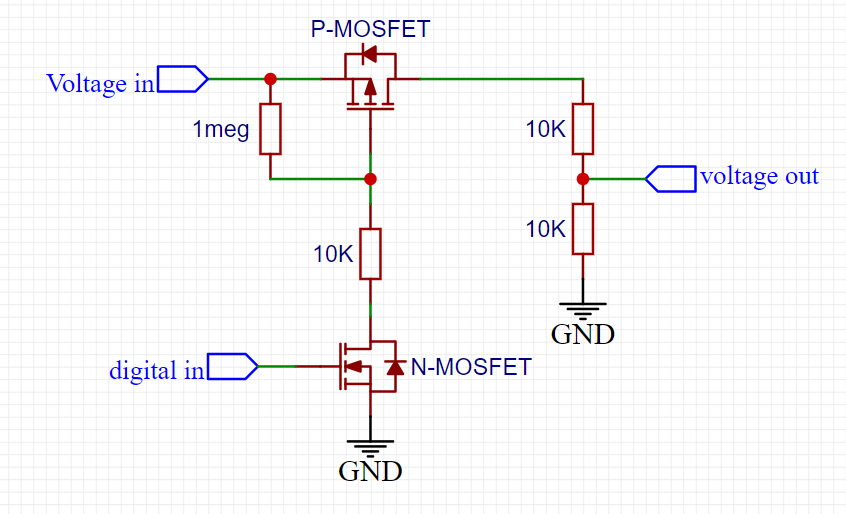
\includegraphics[width=9cm]{messMitTeiler.PNG}
		\caption{\label{pic:messrichtigmitteiler} Mosfetschaltung zur aktivierbaren Spannungsmessung mit Spannungsteiler}
	\end{center}
\end{figure}
\newpage
In \autoref{pic:messrichtigmitteiler} ist zu sehen, dass die Schaltung um einen Spannungsteiler erweitert wurde. Da beide Widerstände den gleichen Wert haben, kann zwischen ihnen die halbierte Spannung gemessen werden. 
Um in der Software die richtige Spannung der Zelle zu erhalten, muss der gemessene Wert verdoppelt werden. Zieht man nun die Spannung der ersten Zelle ab, ergibt das den richtigen Wert für die zweite Zelle.

\chapter{Konzeption des verteilten Systems auf der Hochbahn}
\label{sec:software}
Die Software der Anlage lässt sich in die zwei Bereiche \textit{Webserver im Heimnetzwerk} und \textit{Client auf der Hochbahn} gliedern. Der Webserver soll ein Interface für Benutzer der Anlage bereitstellen, auf dem die Hochbahn gesteuert werden kann. 
Der Client bekommt daraufhin Befehle vom Webserver und führt diese, sofern möglich, aus. 

\section{Konzept für die Aufgabenverteilung auf der Hochbahn}
\label{sec:hochbahnAlsClient}
Wie schon in \autoref{sec:konzeptSchnittstellen} aufgeführt, sollte die Software ursprünglich in drei Hauptkomponenten getrennt weden:
\begin{itemize}
	\item ESP32 zur Befehlserkennung und Steuerung der Hochbahn
	\item Arduino Nano zur Motorsteuerung
	\item Arduino Nano zur Ultraschallüberwachung
\end{itemize}
\autoref{sec:konzeptSchnittstellen} stellt das erste Konzept zur Aufteilung der Aufgabenbereiche dar. Nach Evaluierung der hierbei aufkommenden Fehlerquellen sind einige Änderungen getroffen worden.
Ursprünglich sollte der ESP32 die Hauptsteuerung übernehmen. Er sollte Befehle wie \texttt{beschleunigen} oder \texttt{abbremsen auf Geschwindigkeit x} zur Motorsteuerung geben und dabei die aktuelle Position und damit die nächsten Schritte selbst errechnen. Die Erfahrung zeigt jedoch, dass ein ESP32 mit hoher Netzlast oder Verbindungsabbrüchen leicht zum Neustart oder gar Abstürzen neigt. Würde das passieren während die Bahn beispielsweise auf die Endstation zurollt, bekäme die Motorsteuerung nicht rechtzeitig den Befehl zum abbremsen und es käme zu einem Unfall.
Deswegen wurde die Hauptsteuerung an den Arduino Nano, welcher ursprünglich nur den Motor steuern sollte, übergeben. Daraus resultiert das folgende KOnzept für die Aufgabenverteilung auf der Hochbahn:

\subsection{ESP32 als Schnittstelle zum Server}
\label{sec:aufgabeESP}
Der ESP32 nimmt nachwievor Befehle des Webservers entgegen. Er ist ebenfalls mit dem Reedkontakt welcher über Magneten an der Schiene die Position aktualisiert, verbunden. Das ermöglicht ihm, unabhängeíg von der Hauptsteuerung Positionsmeldungen an den Webserver schicken. Zudem gibt er Befehle an die Hauptsteuerung, welche sich allerdings auf die anzufahrende Position beschränken. Die Fahrt selbst wird vom Arduino Nano gesteuert:

\subsection{Arduino Nano als Hauptsteuerung}
\label{sec:aufgabeArduinoNanoMotor}
Die Hauptsteuerung erhält vom ESP32 Anfahrpositionen. Über den Interrupt des Reedkontakts, wie auch beim ESP (\autoref{sec:aufgabeESP}), ist dem Arduino die aktuelle Position bekannt. Daraufhin soll ein individuelles Fahrprogramm des Schemas \textit{Von x nach y} berechnet und ausgeführt werden. Ebenfalls sind zwei analoge Pins angeschlossen, über jene Auskunft über den Ladezustand der Batteriezellen getroffen werden kann. Der zweite an den Arduino angeschlossene Interrupt dient der Kollisionserkennung. Dieser wird vom Arduino, welcher die Ultraschallsensoren steuert, übermittelt. Dabei gibt die Länge des Pulses Auskunft darüber, um welche Art der Kollisionserkennung es sich handelt.

\subsection{Arduino Nano zur Ultraschallüberwachung}
\label{sec:aufgabeArduinoNanoUltraschall}
Dieser Arduino hat nur die Aufgabe beide Ultraschallsensoren (jeweils einer auf jeder Seite des Tabletts) zu überwachen und mit einem Pin Auskunft darüber zu geben, welches Warn- oder Schutzfeld verletzt wurde. Da nur ein Pin zur Verfügung steht, bestimmt die Länge des \texttt{High}-Signals die Art der Kollisionserkennung.

\section{Protokoll der Seriellen Schnittstelle}
Die Datenübertragung erfolgt, wie in \autoref{sec:konzeptSchnittstellen} erwähnt, über \acrshort{uart}. In den Grundlagen unter TODO ist zu lesen, dass \acrshort{uart} die Daten byteweise überträgt. Die Bytes werden in einen Puffer geschrieben und können auf Anwendungsschicht Byte für Byte ausgelesen werden. Daher ist es logisch, das Protokoll so zu konzeptionieren, dass möglichst wenige, bzw. pro Befehl nur ein Byte verwendet wird. 

\subsection{Anfragen- und Befehlsarten}
Anfrage- oder Befehlsnachrichten können auf zwei Wegen erfolgen: Von ESP zu Arduino und umgekehrt. Es gibt insgesamt fünf Kategorien von Datenübertragungen:

\begin{itemize}
	\item Positionsabfrage zur Positionssynchronisation,
	\item Fahrbefehl von ESP zu Arduino mit anzufahrender Position,
	\item Akkumeldung von Arduino zu ESP,
	\item Positionsmeldung zur Positionssynchronisierung
	\item und Akzeptieren oder Ablehnen von Fahrbefehlen.
\end{itemize}

Da es pro Übertragungsweg nur maximal drei verschiedene Arten von Nachrichten sind, ergeben sich zwei Bits für den Header des Protokolls. Dadurch kann festgestellt werden, um welche Art von Nachricht es sich handelt.
Soll eine Nachricht nur ein Byte groß sein, bleiben somit sechs Bits für den Body der Nachricht. 
\autoref{tab:header} zeigt den Header der verschiedenen Nachrichtenarten:
%---------------TODO-------------
\begin{table}[h]
	\begin{center}
		\begin{tabular}{m{2cm} | m{2cm} | m{5cm} | m{5cm}}
			Bit \texttt{0} & Bit \texttt{1} & Bedeutung & Nachrichtenweg\\
			\hline 
			\texttt{0} & \texttt{0} & Positionsabfrage  & ESP      ->  Arduino\\
			\hline 
			\texttt{0} & \texttt{0} & Akkumeldung & Arduino  ->      ESP\\
			\hline 
			\texttt{0} & \texttt{1} & Fahrbefehl & ESP      ->  Arduino\\
			\hline 
			\texttt{1} & \texttt{0} & Positionsmeldung & Arduino  ->      ESP\\
			\hline 
			\texttt{1} & \texttt{1} & Befehlsakzeptierung & Arduino  ->      ESP\\
		\end{tabular}
	\end{center}
	\caption{\label{tab:header}Header des Nachrichtenprotokolls}
\end{table}

\subsection{Nachrichtencontext (Body)}
Der Body einer übertragenen Nachricht wird je nach Header anders interpretiert. Beispielsweise können übertragene Werte den aktuellen Ladezustand des Akkus oder die Position der Hochbahn bedeuten. 
In folgender Tabelle sind die verschiedenen Arten des Contexts mit entsprechendem Header aufgelistet:

\begin{table}[h]
	\begin{center}
		\begin{tabular}{r | l | l}
			Body & Header & Bedeutung \\
			\hline
			\texttt{000000} - \texttt{001111} & \texttt{10} & Positionsmeldungen von 0 - 15 \\
			\hline
			\texttt{000000} - \texttt{001111} & \texttt{01} & Fahrbefehle von 0 - 15 \\
			\hline
			\texttt{000000} & \texttt{00} & Positionsabfrage \\
			\hline
			\texttt{000000} - \texttt{001111} & \texttt{00} & Akkumeldung von 0-100\% in ~ 6\% Schritten \\
			\hline
			\texttt{000001} und \texttt{000010} & \texttt{11} & Befehlsakzeptanz \texttt{01} = ja; \texttt{10} = nein\\  
		\end{tabular}
	\end{center}
	\caption{\label{tab:body}Body des Nachrichtenprotokolls}
\end{table}

\subsection{Tail}
In \autoref{tab:body} istzu erkennen, dass nie die letzten beiden Bits verwendet werden. Diese dienen dazu, den Transportweg der Nachricht zu erkennen. Dadurch ist eine Aussagen darüber, ob es sich beim Header \texttt{00} um eine Positionsabfrage oder eine Akkumeldung handelt, möglich.
Ist das Tail mit \texttt{01} gekennzeichnet, handelt es sich um eine Nachricht von ESP32 zu Arduino. \texttt{10} steht für die umgekehrte Richtung.
In folgendem sind zwei Beispielnachrichten genannt, welche der Definition des Protokolls entsprechen:

\begin{center}
	\begin{itemize}
		\item \texttt{01000000}; Positionsabfrage von ESP zu Arduino
		\item \texttt{10001110}; Positionsmeldung mit dem Context: Position 3  
	\end{itemize}
\end{center}
\newpage


\chapter{Konzeptionierung der einzelnen Softwarekomponenten der Hochbahn}
\section{Zustandsautomat des ESP32}
\label{sec:stateESP}
Die Software des EPS32 wird als Zustandsautomat realisiert. Dieser hat, wie schon in \autoref{sec:aufgabeESP} erwähnt, die Aufgabe zwischen Server und Hauptsteuereung auf dem Arduino zu vermitteln.

\begin{figure}[h]
	\begin{center}
		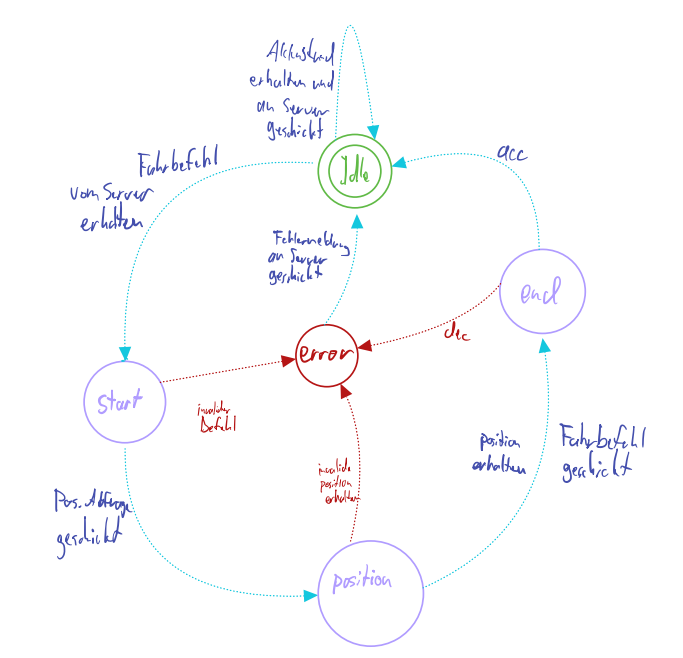
\includegraphics[width=14cm]{stateMaschineESP.PNG}
		\caption{\label{pic:statemaschineESP}Zustandsautomat des ESP32 grafisch dargestellt}
	\end{center}
\end{figure}

In \autoref{pic:statemaschineESP} sind alle Zustände, sowie Zustandsübergänge gezeigt. Das Programm startet im Zustand \texttt{IDLE}. Ein Zustandswechsel kann durch eine Nachricht vom Server oder Arduino erfolgen. Eine Akkumeldung des Arduinos führt zu einer Akkumeldung zum Server und bleibt dabei im Zustand \texttt{IDLE}.
Erhält der ESP einen Fahrbefehl vom Server, wechselt er zu Zustand \texttt{START}. Dieser beginnt eine Folge von Nachrichten und Handlungen mit dem Ziel \textit{die aktuelle Position der Hochbahn zu synchronisieren und den Fahrbefehl auszuführen}. \\
Dazu wird erst eine Positionsanfrage an den Arduino geschickt und in den Zustand Position gewechselt. Erhält der ESP daraufhin die Position kann er die eigens gespeicherte aktualisieren und den Fahrbefehl an den Arduino schicken. Ist dies geschehen, befindet der ESP sich im End-ZUstand und wartet auf eine Akzeptierung seitens des Arduinos. Wird akzeptiert, befindet sich der ESP wieder im IDLE-Zustand und die Kette beginnt wieder von vorne. Sollte der Arduino die Anfrage ablehnen oder sonst auf diesem Weg irgendwas schiefgehen, wird die Kette unterbrochen und in den Error-Zustand gewechselt. Dieser kann mittels des vorherigem Zustand eine Fehlermeldung an den Server schicken, welche dem Nutzer angezeigt wird. Daraufhin kann ein neuer Fahrbefehl oder Akkuzustand empfangen werden. 

\section{Zustandsautomat der Hauptsteuerung}
\label{sec:stateARD}
Ähnlich wie in \autoref{sec:stateESP} wird auch die Software der Hauptsteuerung (Arduino) als Zustandsautomat realisiert. 
Der Automat ist in \autoref{pic:statemaschineARD} gezeigt.

\begin{figure}[h]
	\begin{center}
		\includegraphics[width=10cm]{stateMaschineARD.pdf}
		\caption{\label{pic:statemaschineARD}Zustandsautomat der Hauptsteuerung als Grafik}
	\end{center}
\end{figure}
\newpage
Zu sehen ist dabei wieder eine Kreisstruktur, bei der die einzelnen Zustände über ERROR unterbrechen und wieder in IDLE rücksetzen können. Der generelle Ablauf welcher in einer erfolgreich ausgeführten Fahr mündet ergibt sich wie folgt:

\begin{center}
	\begin{itemize}
		\item 1. Eine Nachricht mit Positionsanfrage vom ESP wurde empfangen,
		\item 2. Die aktuelle Position wurde zurückgeschickt und ein Befehl wird erwartet.
		\item 3. EIn Fahrbefehl wurde empfangen und akzeptiert.
		\item 4. Die gewünschte Position wurde angefahren.
	\end{itemize}
\end{center}

Zusätzlich werden im IDLE-Zustand die Batteriespannungen überprüft um rechtzeitig zur Ladestation zu fahren, falls sie zu leer sind. In diesem Fall schaltet sich die Bahn ab, sobald sie beim Laden angedockt ist. TODO IN GRAFIK!! Dieser Vorgang wird ebenfalls ausgelöst, falls über einen längeren Zeitraum keine Fahrbefehle erhalten wurden.

\chapter{Konzeptionierung der Fahrfunktion}
Die Hauptfunktion dieser Methode lässt sich mit folgendem Satz zusammenfassen: \textit{Die Bahn fährt von A nach B.} B ist in diesem Fall die anzufahrende Position, welche vom Server übermittelt wurde. Mit Acht Abschnitten auf der Strecke und der Möglichkeit jeden Abschnitt von jedem Abschnitt aus anzufahren ergeben sich 56 individuelle Fahrprogramme. Eine Möglichkeit wäre, jedes dieser Fahrprogramme einzeln auszuprogrammieren. Ein viel eleganterer Weg ist jedoch, den Arduino selbst für jede Fahrt das Fahrprogramm bestimmen zu lassen. 

\section{Regeln zur bestimmung des Fahrprogramms}
Auf der Strecke gibt es zwei unterschiedlich anzufahrende Positionen:
\begin{center}
	\begin{itemize}
		\item Ein Abschnitt auf der Strecke
		\item und eine der beiden Endpositionen.
	\end{itemize}
\end{center}
Der unterschied liegt darin, dass die Bahn bei einer der beiden Endpositionen exakt am Magneten anhalten muss, während bei Anfahrten von Aschnitten ledigliche zwischen zwei Magneten zu Stoppen ist. Die Geschwindigkeit muss also bereits vor eintreten in den letzten Abschnitt so gering sein, dass innerhalb des Abschnittes angehalten, bzw. der letzte Magnet angefahren werden kann.

\chapter{Umsetzung}
\label{cha:umsetzung}
In diesem ersten Teil der Studienarbeit stand die Konzeptionierung in \autoref{cha:konzeptionierung} im Vordergrund. Auf dieses Kapitel aufbauend soll der aktuelle Stand der Umsetzung beschrieben werden. Dieser beschränkt sich bislang auf die Motorsteuerung in \autoref{sec:motorsteuerung} sowie die Getriebekonstruktion in \autoref{sec:getriebekonstruktion}.
\newpage
 
\section{Motorsteuerung}
\label{sec:motorsteuerung}
Die Motorsteuerung ist auf einem Arduino Nano ausgelagert. Der Hochbahncontroller ESP32 kann der Steuerung Befehle erteilen und erhält die aktuelle Geschwindigkeit. In \autoref{pic:motorsteuerung} ist schematisch der Steuerungsablauf  dargestellt. 

\begin{figure}[h]
	\begin{center}
		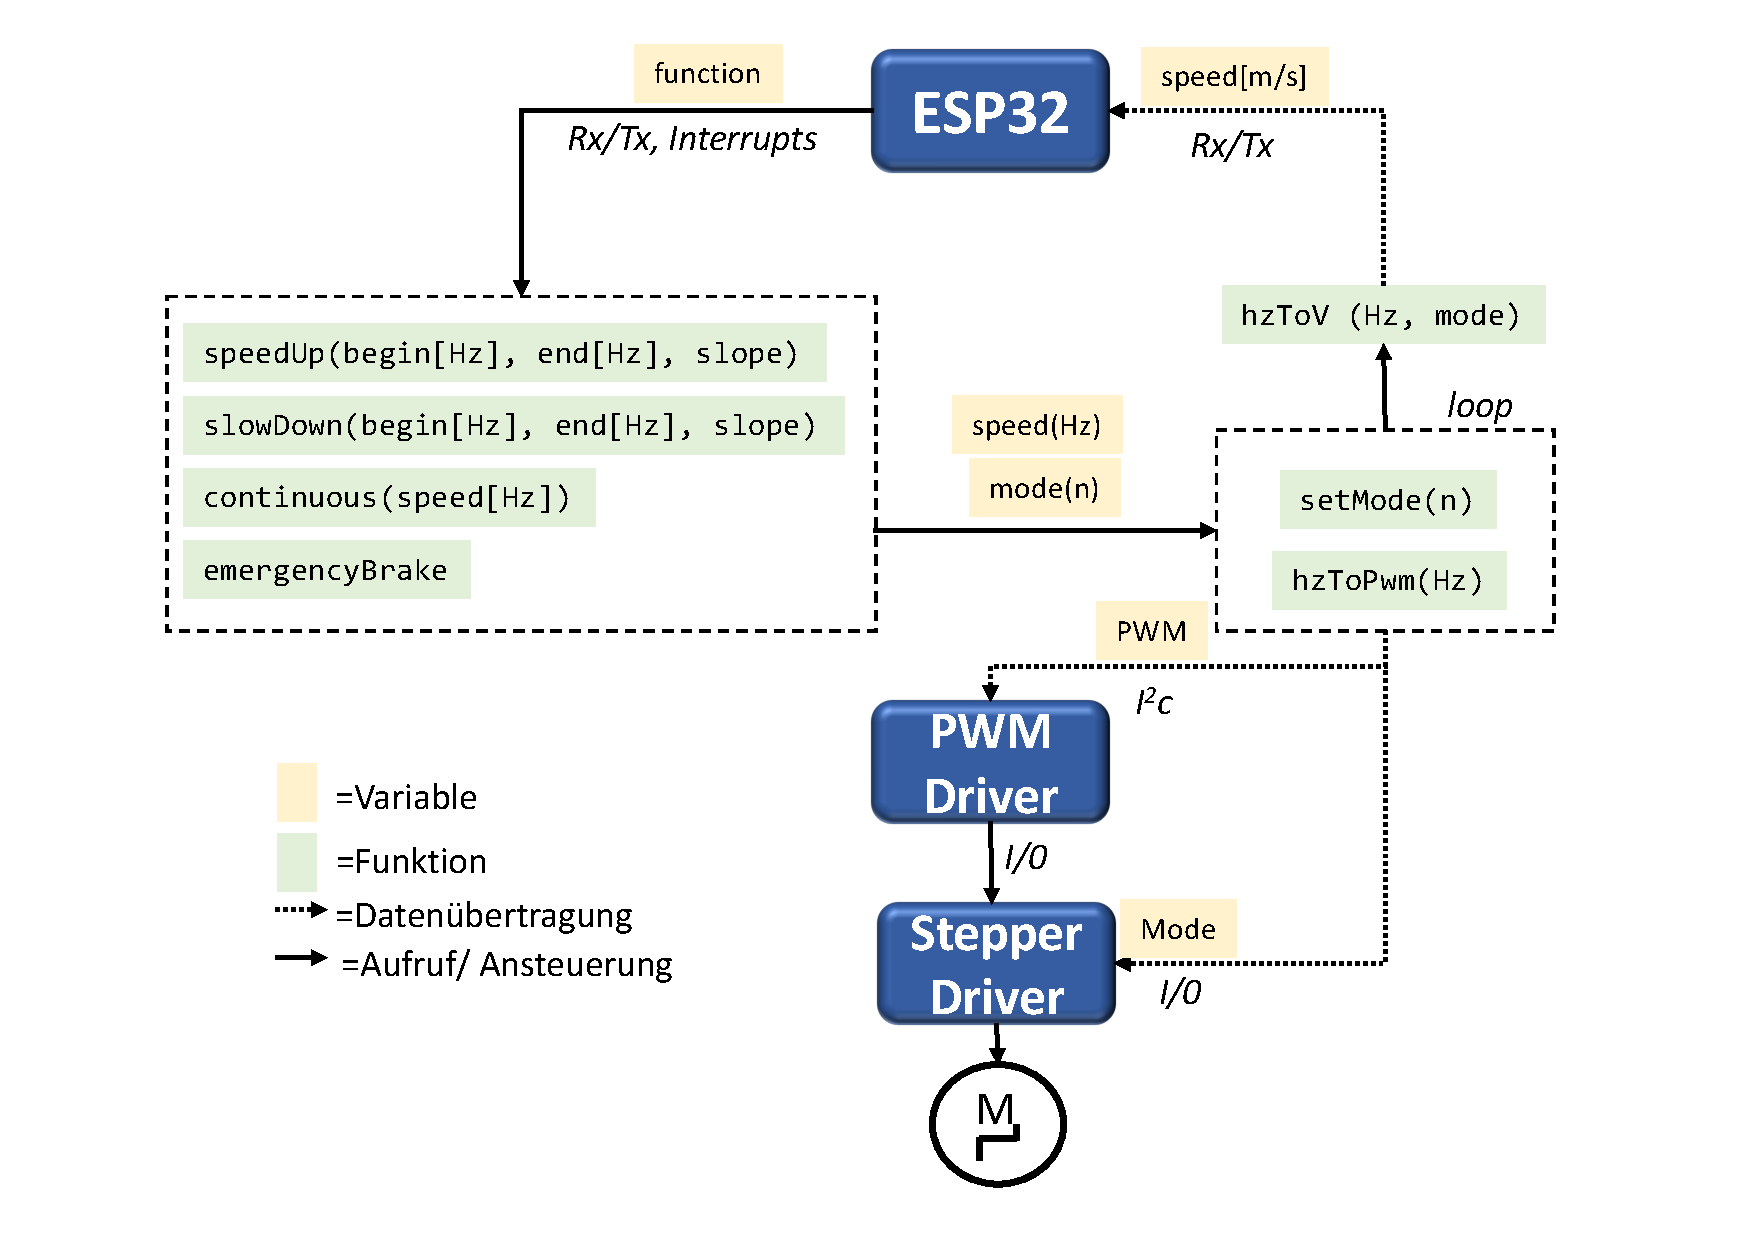
\includegraphics[width=16cm]{motorsteuerung.pdf}
		\caption{Schematische Übersicht der Motoransteuerung}
		\label{pic:motorsteuerung}
	\end{center}
\end{figure}



Für die Motorsteuerung können vom ESP32 Funktionen im Skript ausgeführt werden. Für den Brems- und Beschleunigungsvorgang dienen die beiden Funktionen \textit{ speedUp} und \textit{slowDown}. Als Parameter werden die Start- und Enddrehzahl in $Hz$ sowie der Gradient mitgegeben. Bei einer Fahrt mit gleichbleibender Geschwindigkeit wird \textit{continuos} mit Drehzahlparameter in $Hz$ ausgeführt. Wird das Schutzfeld verletzt, löst der ESP32 die \textit{emergencyBrake} Funktion aus. Die Befehle werden über serielle Kommunikation mit \acrshort{uart} versendet. Der Nothalt wird durch einen Interrupt am Arduino Nano ausgelöst. \\
\newpage

Im Skript sind die beiden Variablen Drehzahl $speed$ und Schrittmodus' $mode$ global angelegt. Diese werden von den Steuerungsfunktionen verändert. Die Variablen dienen den Funktionen $setMode, hzToPwm$ und $hzToV$ als Grundlage. Diese werden in einer Schleife ausgeführt. $setMode$ stellt den Schrittmodus am Motortreiber über die \acrshort{gpio}-Pins am  Treiber ein. $hzToPwm$ berechnet anhand der aktuellen Drehzahl die Geschwindigkeit in $\frac{m}{s}$. Der Wert wird über die serielle Schnittstelle an den ESP32 zurückgegeben. Die Funktion $hzToPWM$ bestimmt aufgrund der geforderten Drehzahl den \acrshort{pwm}-Wert. Der Wert wird über $I^2C$ an einen  \acrshort{pwm}-Treiber übergeben und dient als Takt für den Schrittmotortreiber. \\

Während erster Versuche wurde der Takt für den Schrittmotortreiber durch den Mikrocontroller generiert. Dabei zeigte sich, dass die maximale Taktrate stark von der Auslastung des Mikrocontrollers abhängt. Durch die Verwendung des \acrshort{pwm}-Treibers wird die Takterzeugung ausgelagert. Dafür sind die Zeiten $T_{off}$ und $T_{on}$ des \acrshort{pwm}-Signals dieselben. Es wird lediglich die Frequenz des Signals verändert. 
 \newpage

\section{Getriebekonstruktion}
\label{sec:getriebekonstruktion}
Wie im Konzeptionierungsteil \ref{sec:getriebekonstruktion} beschrieben, soll für die Kraftübertragung des Motors auf die Schiene ein Riemengetriebe verwendet werden. In diesem Kapitel wird die Konstruktion des Getriebes beschrieben. In \autoref{pic:getriebe} ist eine Übersicht des Getriebes dargestellt. Auf die Bauteile wird nachfolgend genauer eingegangen. 

\begin{figure}[h]
	\begin{center}
		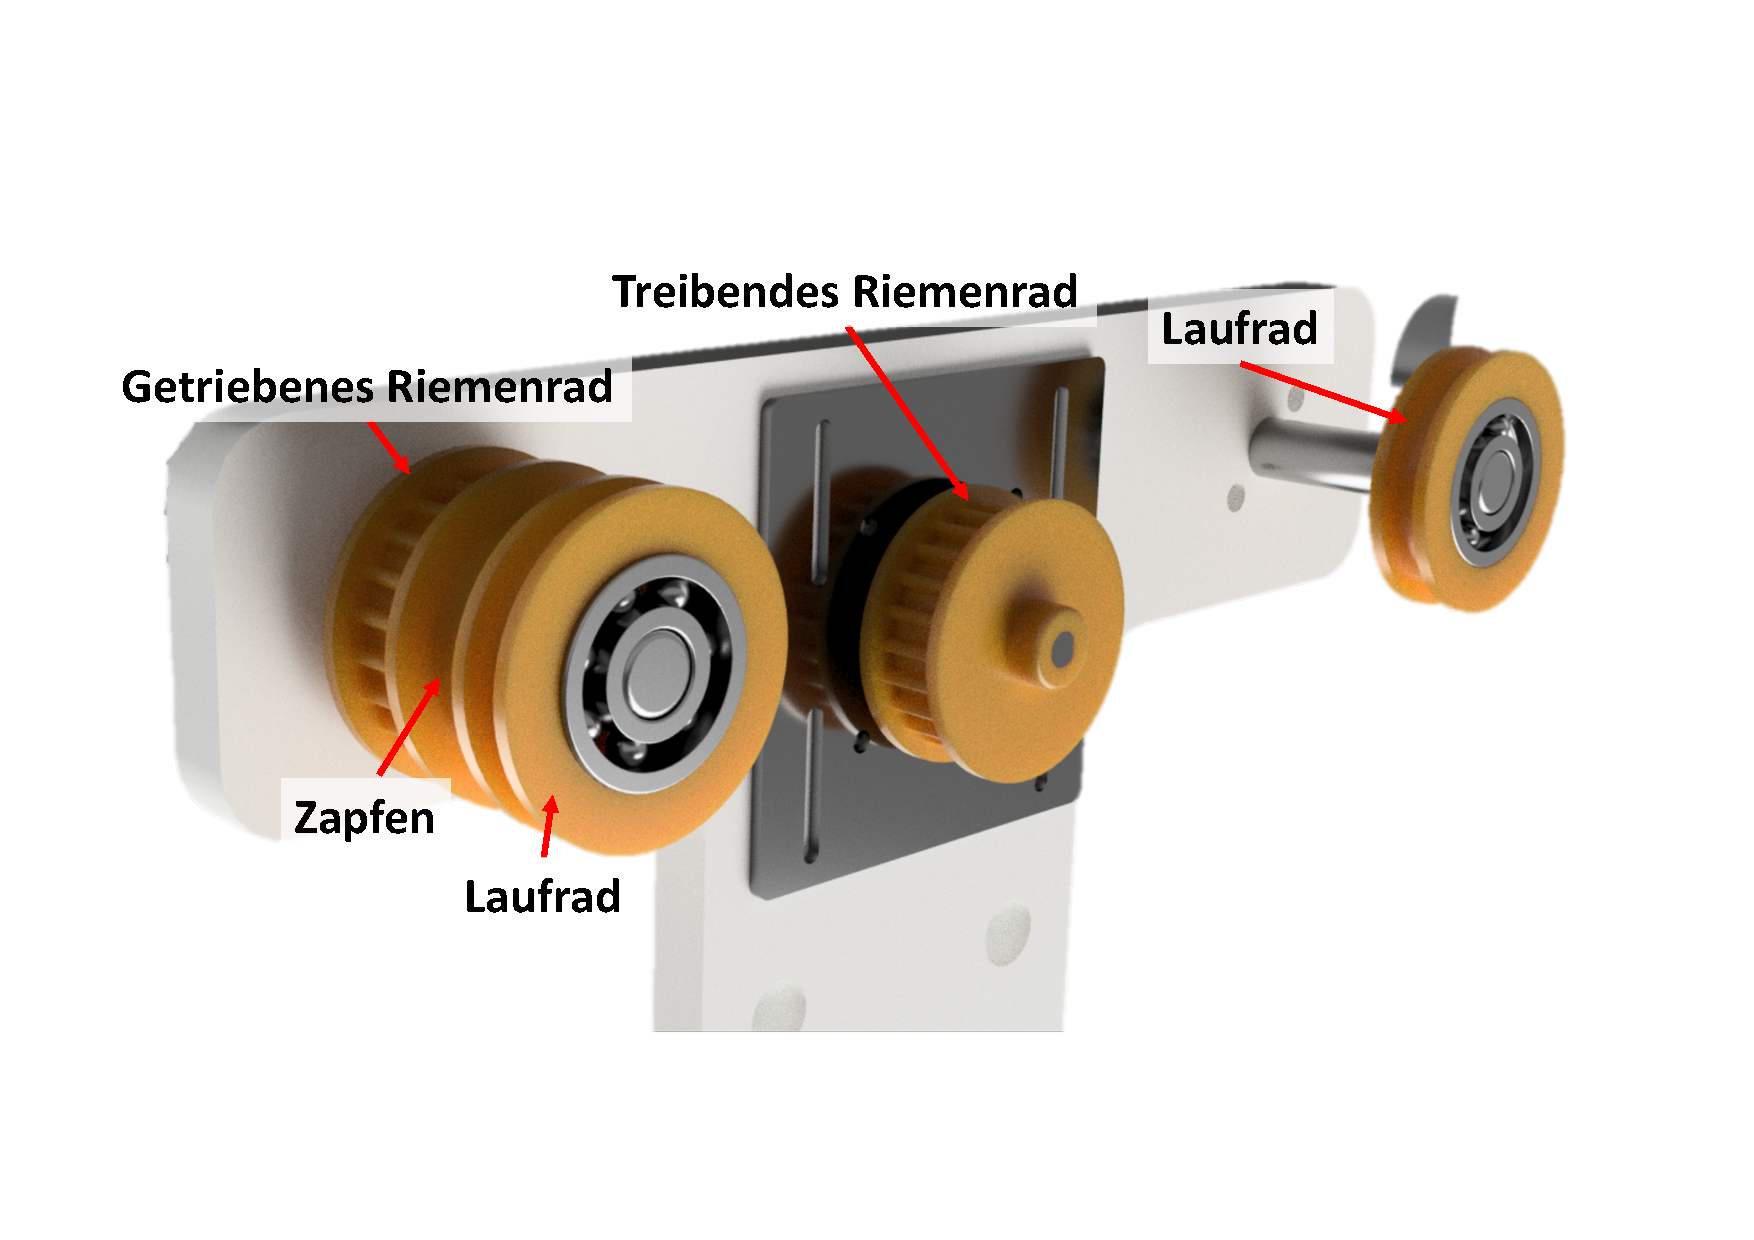
\includegraphics[width=12cm]{getriebe.pdf}
		\caption{Gerenderte Konstruktionsansicht der Getriebekonstruktion}
		\label{pic:getriebe}
	\end{center}
\end{figure} 



\textbf{Das Laufrad}\\
Beim Laufrad beträgt der Durchmesser der Lauffläche $d=34mm$ bei einer Breite $b=5mm$. Für die Führung auf der Schiene sorgen seitliche Ränder. Diese besitzen eine Breite $b_R=2mm$ sowie einen Durchmesser $d=40mm$. Die Laufräder werden mit einem Rillenkugellager 6000 Welle gelagert. Das Lager wird mit Übermaßpassung verbaut. Das Laufrad ist in \autoref{pic:laufrad}dargestellt. \\

\begin{figure}[h]
	\centering
	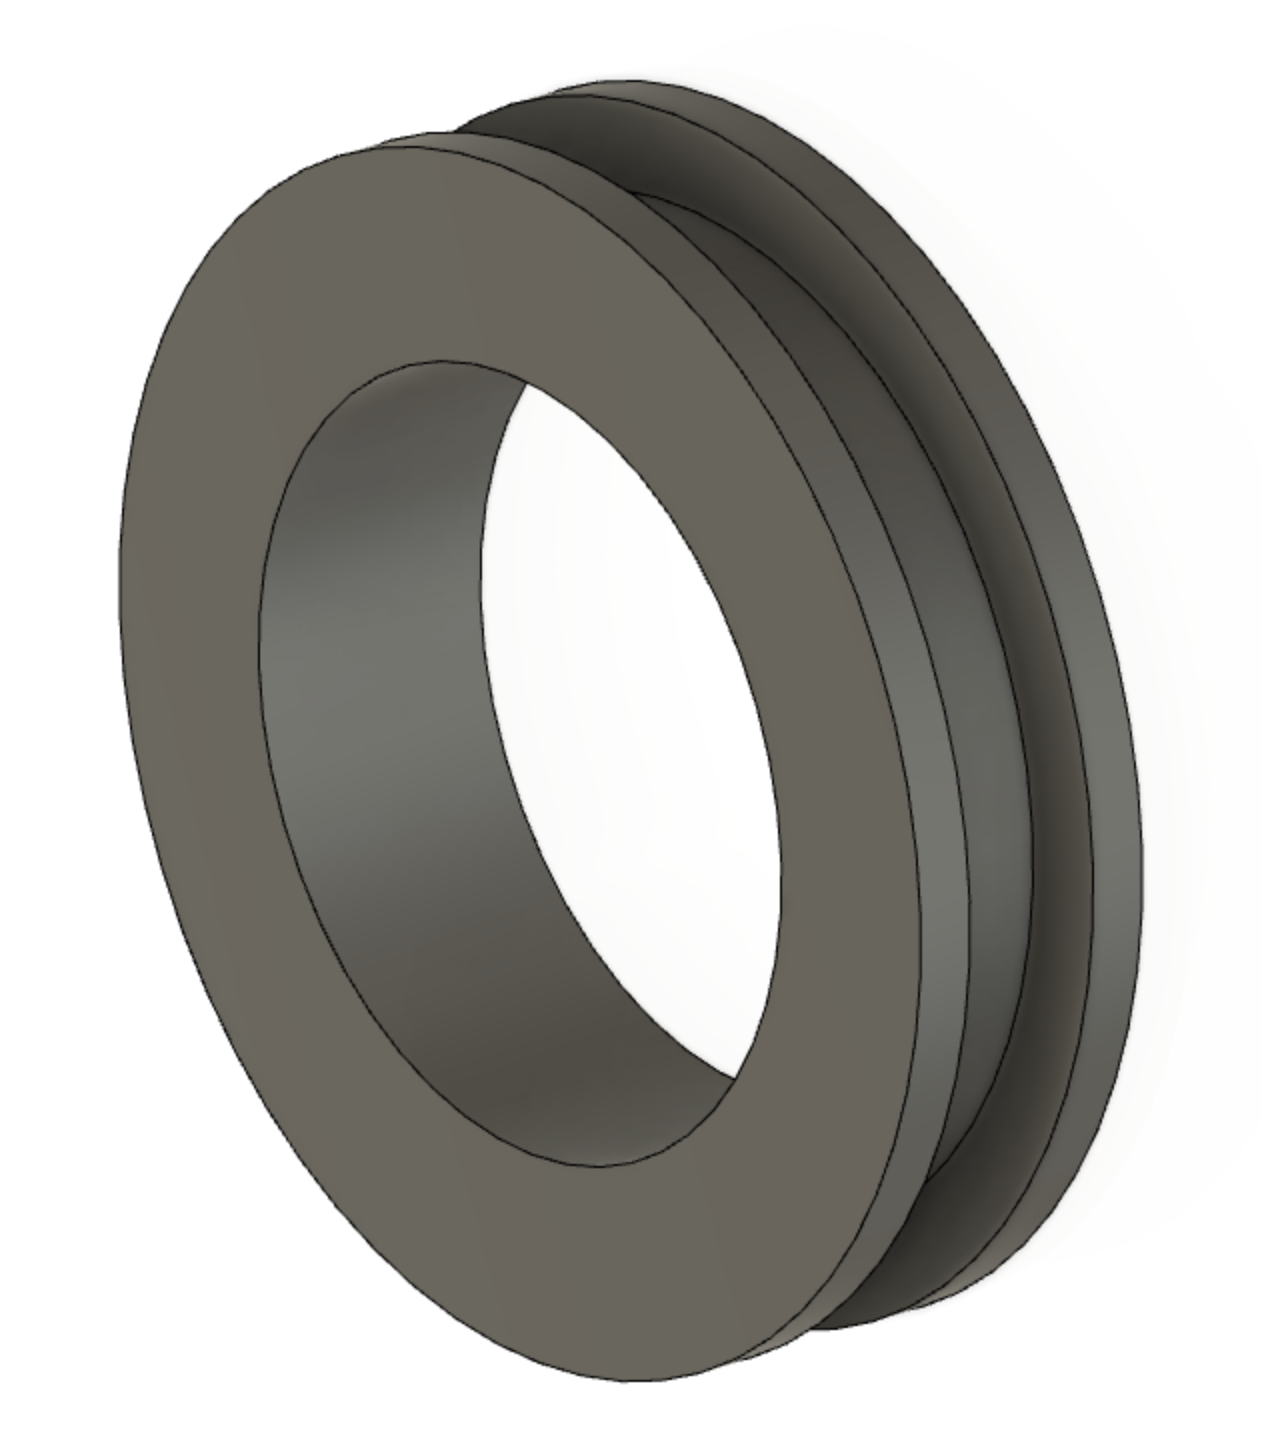
\includegraphics[width=3cm]{laufrad.png}
	\caption{Konstruktionsansicht des Laufrades}
	\label{pic:laufrad}
\end{figure}
\newpage

\textbf{Die Riemenräder}\\   
Das Riemengetriebe besteht aus einem treibenden und getriebenen Riemenrad. Zunächst soll das Zahnprofil der beiden Riemenräder ausgelegt werden. Dafür ist die Grundlage der Zahnflachriemen mit einem äußeren Umfang von $U = 206mm$ und einer Riemenbreite von $b=9,5mm$. Die Zähnezahl des Riemens beträgt $z_R=75$. Folglich ist das Modul $m \approx 5$. \\

 Für das Zahnprofil muss ebenfalls das Modul $m=5$ verwendet werden. Die Zähnezahl wird auf $z=22$ festgelegt. Dadurch ergibt sich für den Kopfkreisdurchmesser $d_Z$ des Profils: 
 
 \begin{align}
 	d_Z =  \frac{m \cdot z}{\pi} = \frac{5 \cdot 22}{\pi} \approx 35,01
 \end{align}


Entsprechend der Abmessungen des Riemens wurde der Durchmesser der Zahnflanken auf 2mm festgelegt.  Das treibende Riemenrad (Ritzel) ist in \autoref{pic:ritzel} dargestellt. Es wird auf die Nabe des Motors gesteckt. Durch die Phase auf der Motorwelle geschieht die Übertragung des Drehmoments formschlüssig.  Das getriebene Riemenrad zeigt \autoref{pic:riemenlaufrad} und ist beidseitig gelagert. Dafür wird ebenfalls das Kugellager 6000 mit Übermaßpassung verbaut.  
 

\begin{figure}[h]
	\centering
	\begin{minipage}[t]{0.45\linewidth}
		\centering
		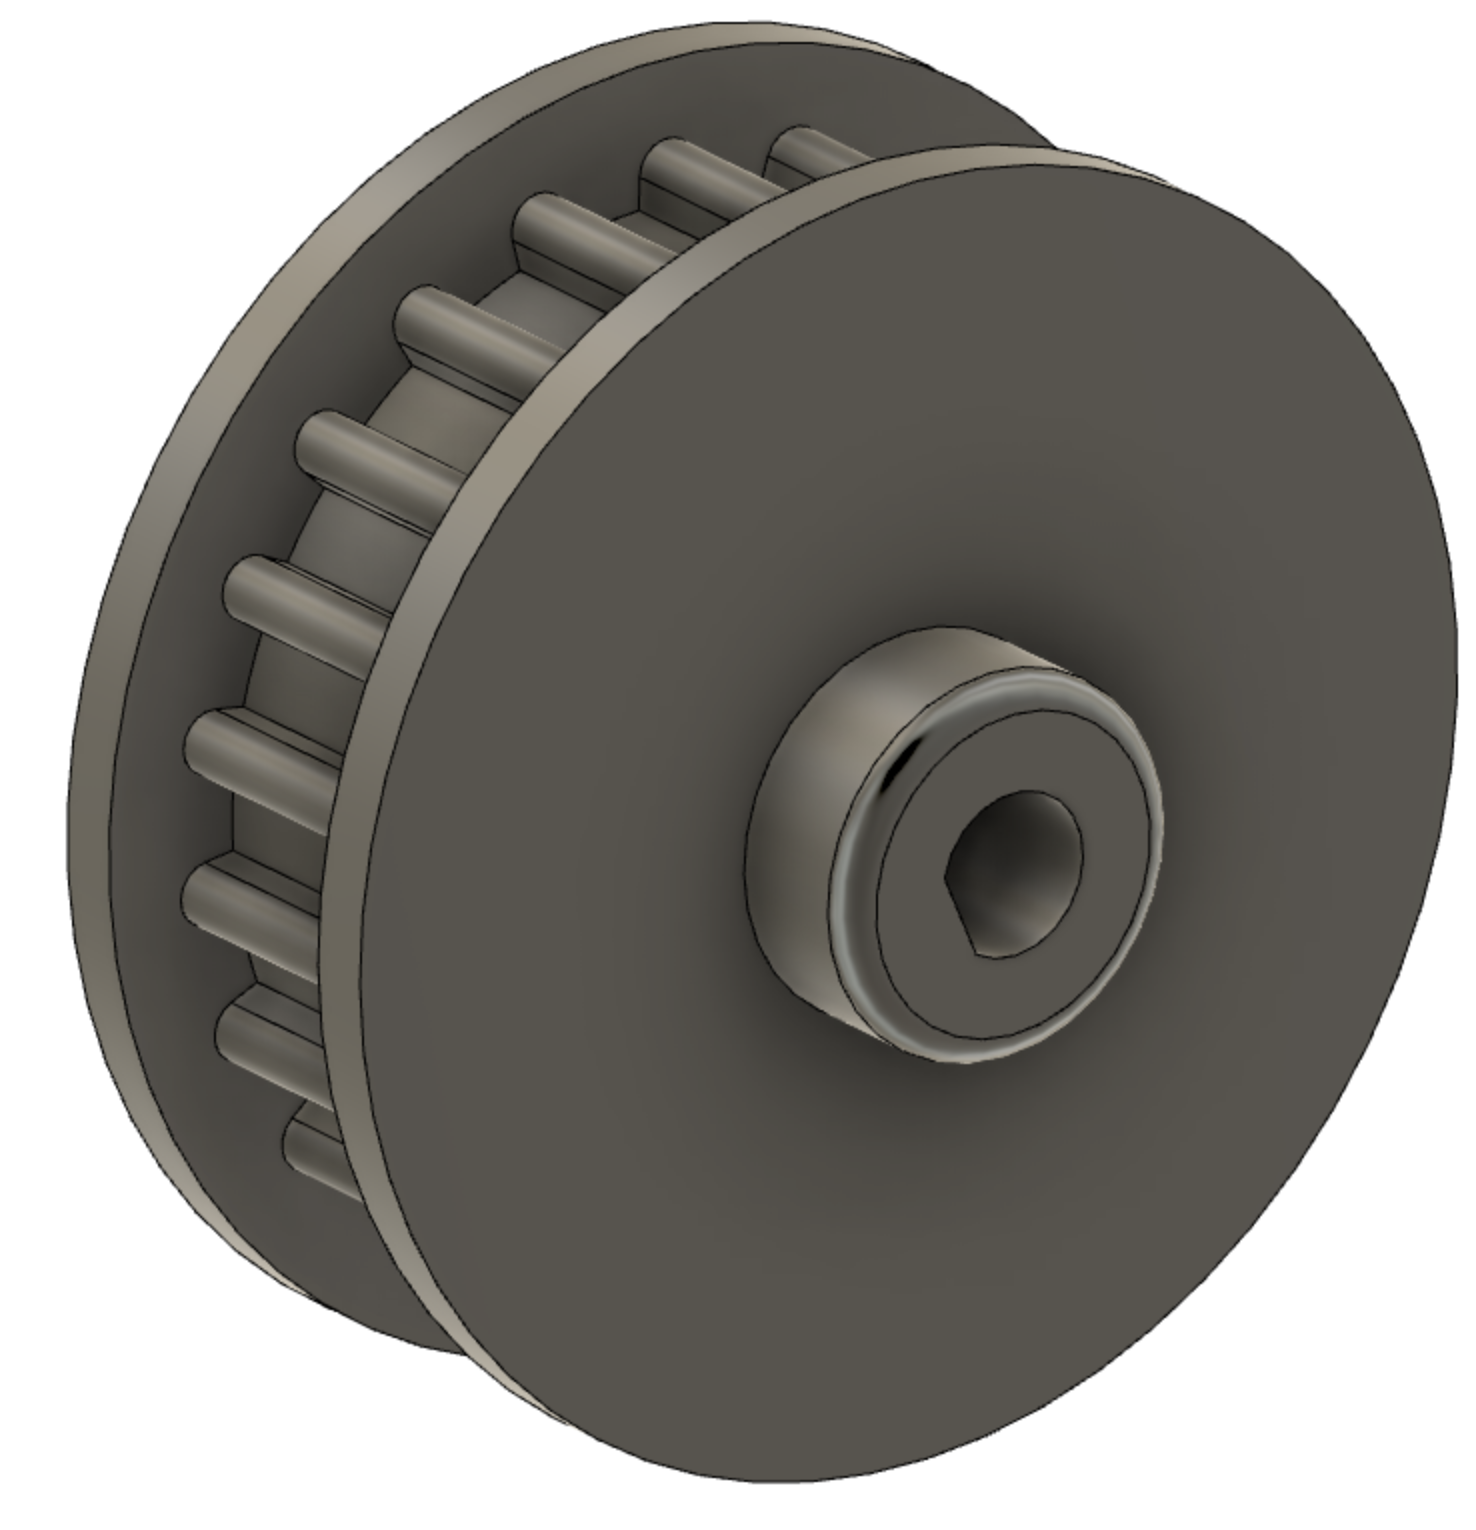
\includegraphics[width=4cm]{ritzel.png}
		\caption{Konstruktion des treibenden Riemenrades (Ritzel)}
		\label{pic:ritzel}
	\end{minipage}
	\hfil	
	\begin{minipage}[t]{0.45\linewidth}
		\centering
		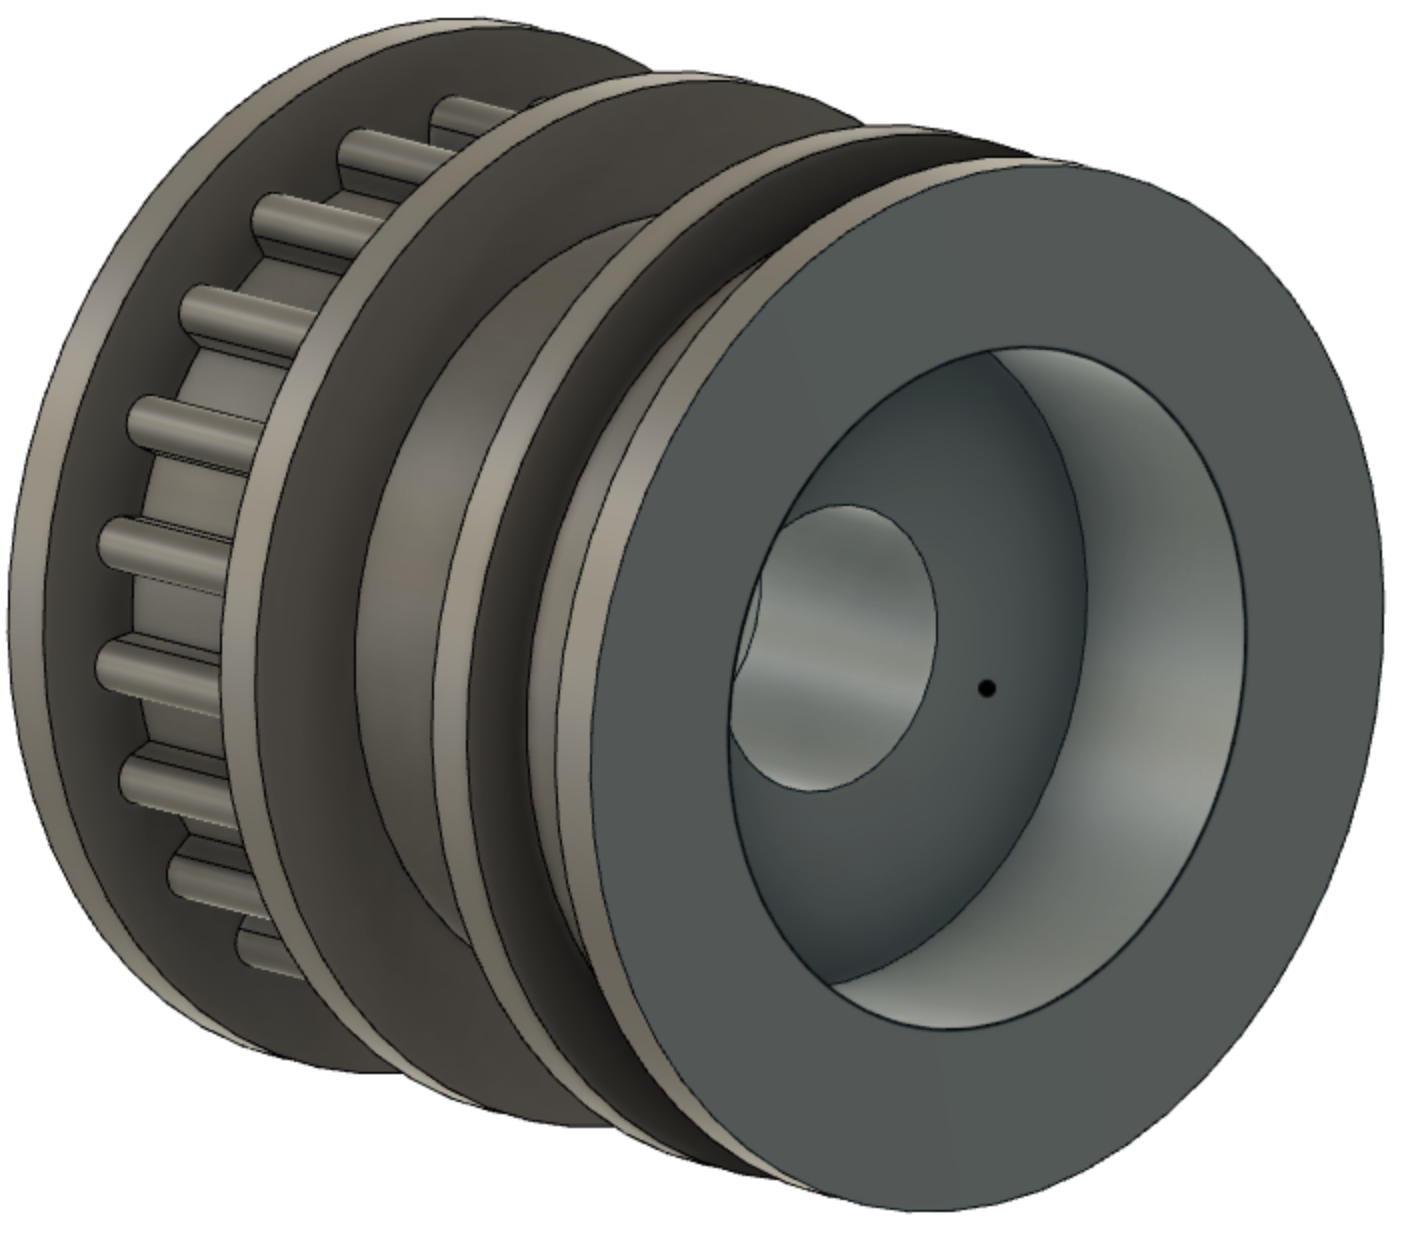
\includegraphics[width=4cm]{riemenlaufrad.png}
		\caption{Konstruktion des getriebenen Riemenrades mit Laufrad}
		\label{pic:riemenlaufrad}
	\end{minipage}	
\end{figure}



\newpage


\textbf{Implementierung des Getriebes}\\
Der äußere Umfang des Riemens beträgt $U = 330mm$. Für die Berechnung des erforderlichen Abstandes $\Delta$ der beiden Wellen zueinander gilt:

\begin{align}
	U = 2 (r \cdot \pi+ \Delta) 
\end{align}

Und damit: 
\begin{align}	
	\Delta = \frac{U - 2r \cdot \pi}{2} = \frac{330mm - 35,01 \cdot \pi}{2} \approx 110mm 
\end{align}

Um den Wellenabstand zu erreichen, wird die Motoraufhängung nach unten entsprechend versetzt. Zusätzlich soll sich die Aufhängung nach der Montage in Y-Richtung justieren lassen. Dadurch kann der Riemen nach dem Einbau auf Spannung gebracht werden. Die Motoraufhängung ist in \autoref{pic:motoraufhaengung} dargestellt. 


\begin{figure}[h]
	\centering
	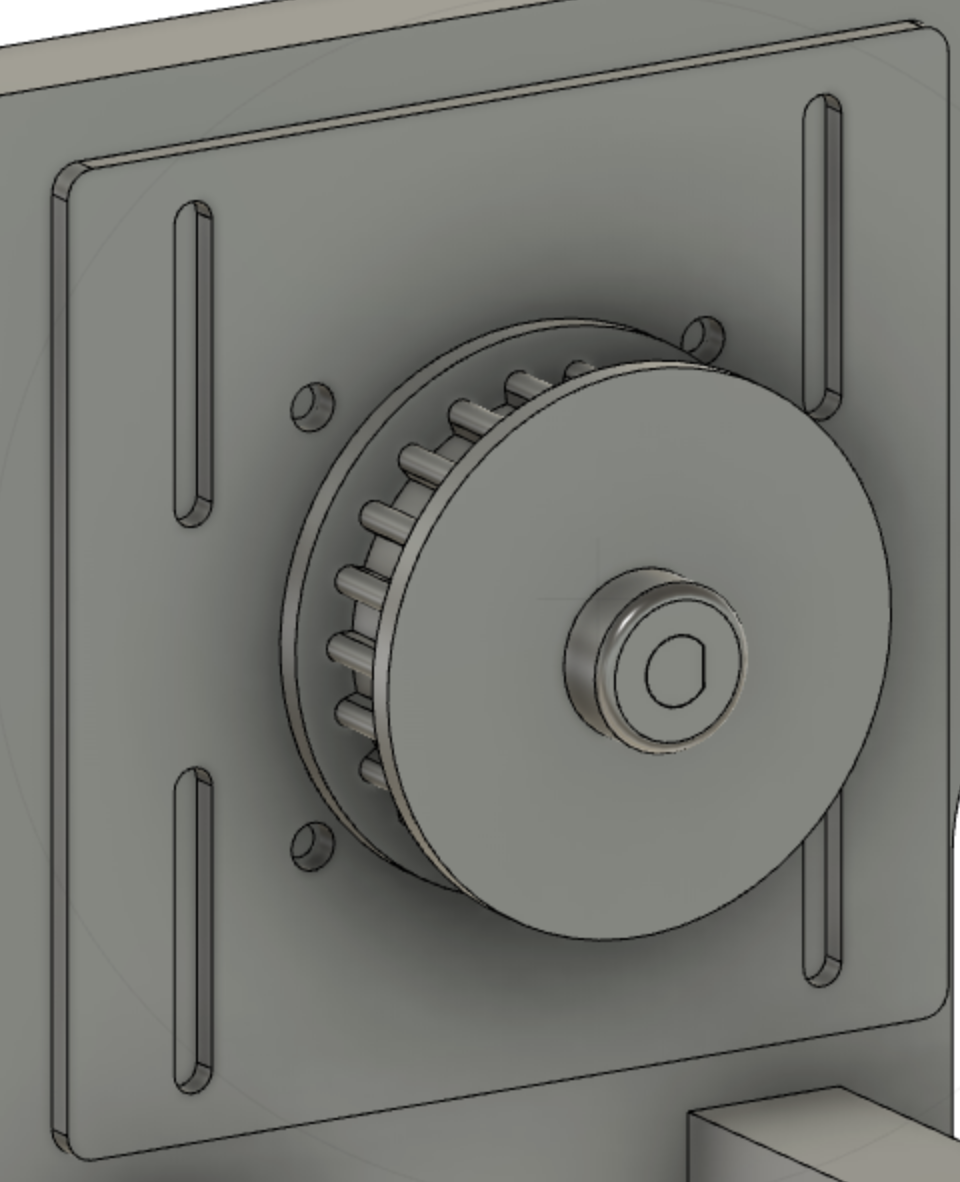
\includegraphics[width=5cm]{motoraufhaengung.png}
	\caption{Konstruktionsansicht der verschiebbaren Motoraufhängung}
	\label{pic:motoraufhaengung}
\end{figure}

Die Wellen werden axial beansprucht. Damit die Befestigung der Welle die axialen Kräfte aufnehmen kann, wird zusätzlich ein Rundmaterial an die Seitenteile montiert. 
\newpage

\chapter{Fertigung der Platine}
\section{Schaltplan}
\label{sec:eCardPlan}
\autoref{pic:schaltplan} zeigt den gesamten Schaltplan für die Platine. Zu sehen sind ESP32, zwei Arduini, sowie Steppertreiber, ein Relais und diverse \textcolor{magenta}{Schraubklemmen} um beispielsweise die beiden \textcolor{orange}{Ultraschallsensoren} anzuschließen. Der Einsatz des \textcolor{red}{Relais} wird in TODO erklärt.Die \textcolor{blue}{Kommunikation zwischen Arduino und ESP} ist in TODO aufgeführt. Unter TODO ist die \textcolor{green}{Mosfetschaltung zur Spannungsmessung} erklärt. All diese Komponenten sind farblich im Schaltplan markiert. In (TODO) wurde das Energieversorgungskonzept erklärt, welches ebenfalls auf der Platine vorhanden sein muss.

\begin{figure}[h]
	\begin{center}
		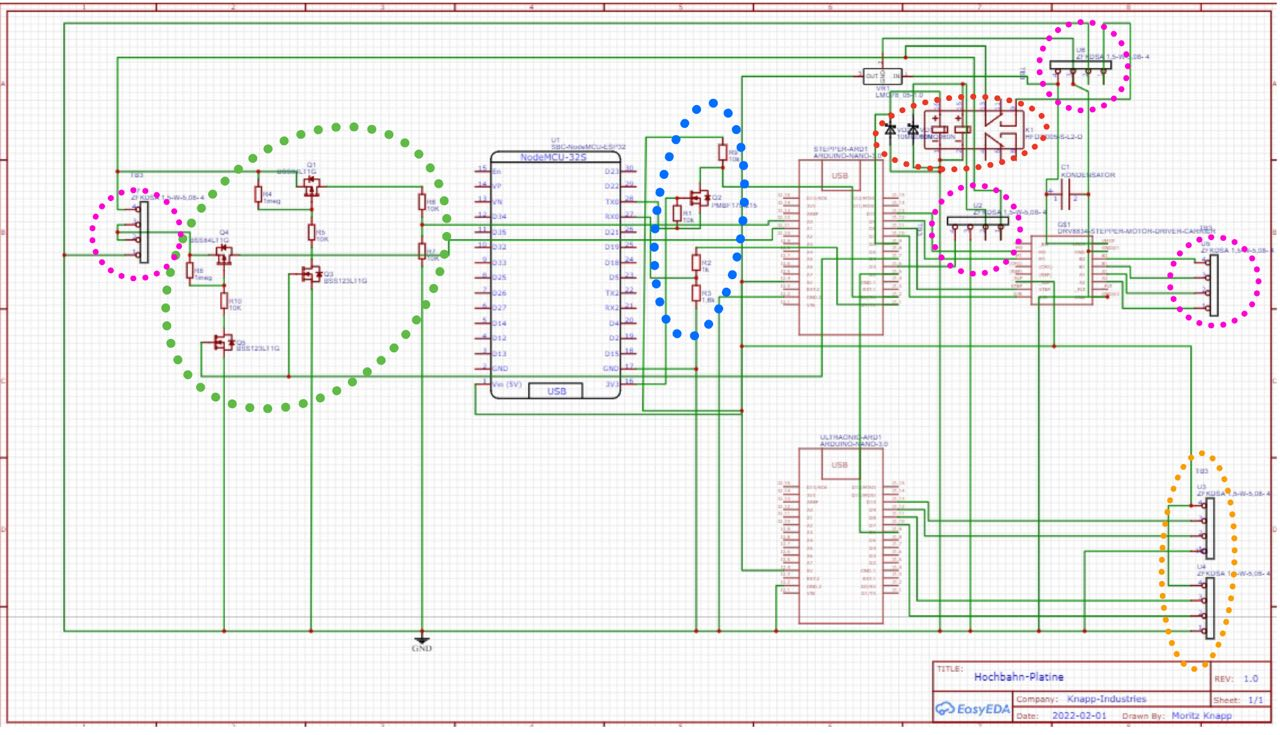
\includegraphics[width=13.3cm]{schaltplan.jpg}
		\caption{\label{pic:schaltplan} Schaltplan der Platine}
	\end{center}
\end{figure}



\section{PCB-Design}
Der fertige Schaltplan aus \autoref{sec:eCardPlan} ist nun in ein fräsbereites Platinen Design umzuwandeln. Um den Fräsaufwand so gering wie möglich zu halten, werden alle elektronischen Verbindungen auf einer Seite platiert. Daraus folgt, dass es zu keinen Überlappungen von Verbindungen geben darf, da sonst der Stromfluss nicht mehr logisch getrennt wäre. Um den Verbindungsaufwand zu verringern, wurde \gls{gnd} auf die Kupferschicht gelegt. Da alle Komponenten den gleichen $-Pol$ haben, müssen sie an der entsprechenden Stelle lediglich an die Schicht gebunden werden, welche somit eine \gls{gnd}-Leitung ersetzt.
\vspace{0.5cm}
\begin{figure}[h]
	\begin{center}
		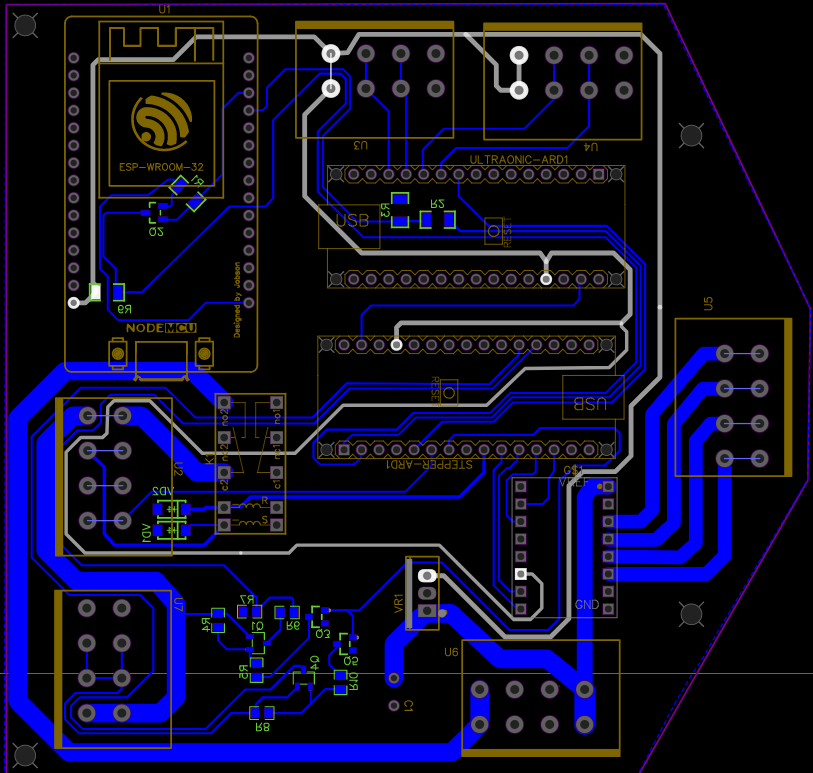
\includegraphics[width = 12cm]{pcbDesign.png}
		\caption{\label{pic:pcbDesign} PCB-Design der Platine}
	\end{center}
\end{figure}

\autoref{pic:pcbDesign} zeigt den PCB-Entwurf für die Hauptplatine. Zu erkennen sind alle zuvor erwähnten Komponenten. Ebenfalls ersichtlich ist (weiß markiert) die 5V Versorgungsleitung. An die unten rechts platzierte Schraubklemme wird der StepUp Wandler für 10V angeschlossen. Dabei ist zu erkennen, dass diese Leitungen besonders dick (2mm) sind. Es handelt sich um die Versorgungsleitung für alle Komponenten, wodurch hier der meiste Strom fließt. Die Dicke verhindert eine Hitzeüberlastung der Leitung. Datensignale sind mit 0.3mm am dünnsten.[TODO: Bib mit dickenliste]
Ebenfalls ersichtlich wird, dass das Relais die Stromleitung der Batterie bereits vor dem Step-Up Wandler trennt. Der Grund dafür ist, dass im ausgeschaltenen Zustand kein Strom aus den Batterien fließen soll, was bei angeschlossenem Wandler der Fall wäre. 

\section{Fertigung}
Gefräst wurde die Platine in der Ausbildungsabteilung der SICK AG. Die bereits mit (todo acr) smd-Teilen bestückte Platine ist in \autoref{pic:ecardCopper} zu sehen. 

\begin{figure}[h]
	\begin{center}
		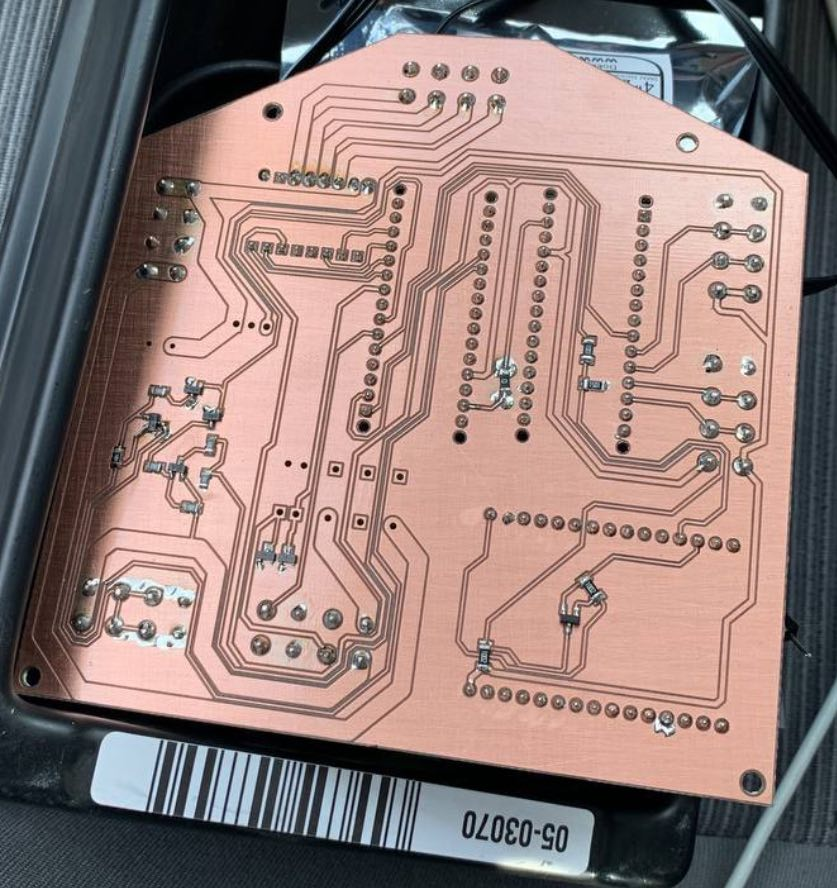
\includegraphics[width = 10cm]{eCardCopper.jpg}
		\caption{\label{pic:ecardCopper}Mit SMD-Teilen bestückte Platine}
	\end{center}
\end{figure}

Nach Verlöten der übrigen Komponenten und Anschluss von Step-Up-Wandler und Batterien konnte die Spannungsversorgung erfolgreich getestet werden. Dass die LEDs der Arduini leuchten und nirgends Überhitzung zu spüren ist zeigt, dass kein Kurzschluss herrscht. Mit dem Multimeter konnten zudem alle Spannungen überprüft werden. In \autoref{pic:ecardLights} ist die fertig bestückte Platine im aktivierten Zustand gezeigt. Die vier Löcher dienen später zur Befestigung in der Elektronikbox.


\begin{figure}
	\begin{center}
		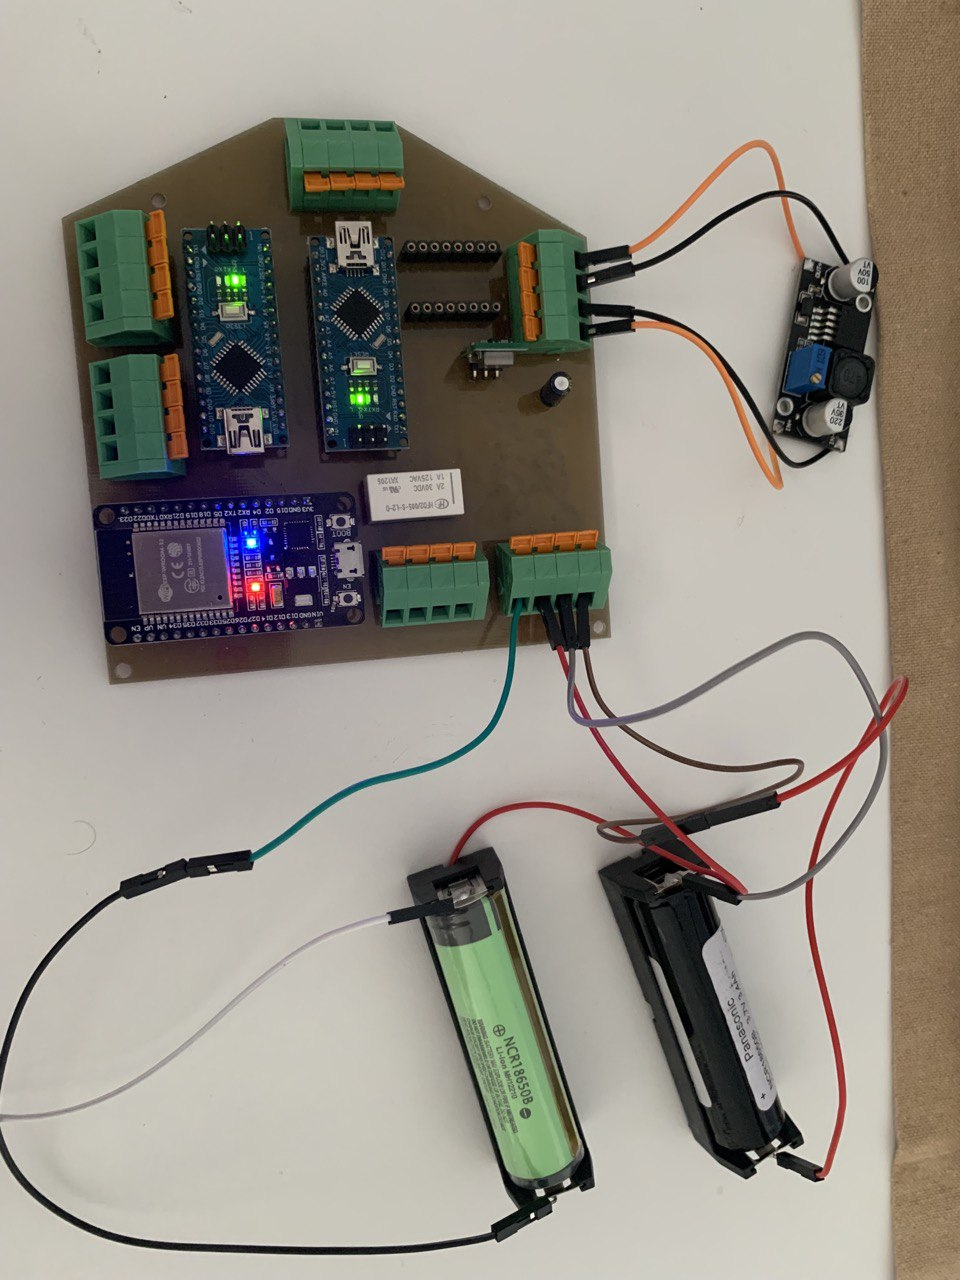
\includegraphics[width=10cm]{ecardLight.jpg}
		\caption{\label{pic:ecardLights}Fertig bestückte Platine}
	\end{center}
\end{figure}

\chapter{Implementierung der Zustandsautomaten}
Im folgenden wird die zuvor unter \autoref{sec:stateESP} konzeptionierte Logik des Zustandsautomaten des ESP32 implementiert.
C++ ist die hierbei verwendete Programmiersprache. Die Idee ist eine State Maschine, die zu jeder zeit einen aktuellen State (\texttt{currentState}) hat, welcher sich in Abhängigkeit von der Eingabe verändert. Beispielsweise soll die Maschine von \texttt{IDLE} nach \texttt{START} wechseln, sofern ein valider Fahrbefehl vom Server erhalten wurde.

\section{Die State Klassen}
Um den Validierungsaufwand innerhalb der Zustandsmaschine zu verringern, d.h. die Maschine muss nicht schauen, was für ein State \texttt{currentState} ist, erben alle Zustände von einer State-Klasse. Somit muss die Maschine später nur wissen, dass sie einen State hat und nicht welchen.
\autoref{code:state.h} zeigt die Header-Datei dieser State-Klasse.

\begin{lstlisting}[language=c, style=dhpaperdefault]
	class State{
		public:
			int driveToPosition;
			String errorMsg;

			virtual int handle(byte);
			virtual int handle(String);
			virtual int handleWithoutParam();
			
			virtual void handle();
	};
\end{lstlisting}
\captionof{lstlisting}{\label{code:state.h} State-Klasse}

Die beiden Klassenvariablen \texttt{driveToPosition} und \texttt{errorMsg} werden verwendet, um State-übergreifende Parameter zu übergeben. Beispielsweise legt ein \texttt{Position-State} als \texttt{errorMsg} den String ''\textit{received invalid position}'' und übergibt diesen an Error-State, welcher die Nachricht an den Server schickt.
Die \texttt{handle}-Methoden geben jeweils ein \texttt{int} zurück, welches signalisiert in welchen Zustandn zu wechseln ist.
Im Folgendem wird die Implementierung der \texttt{handle}-Methoden am Beispiel des Idle-States erklärt:

\subsubsection{Die Idle State Klasse}
\label{sec:IdleState}
Der Zustandsautomat der Hauptsteuerung ist in \autoref{pic:statemaschineARD} zu sehen.
Idle-State hat dabei drei Aufgaben:
\begin{center}
	\begin{itemize}
		\item Batteriezellenzustände überprüfen und an den Esp schicken,
		\item das Zurückfahren zur Ladestation initialisieren falls nötig (Batterie leer)
		\item und das Warten auf eine Positionsanfrage seitens des ESPs.
	\end{itemize}
\end{center}
 Durch diese Aufgaben ergeben sich drei mögliche Zustandswechsel:
 \begin{center}
	\begin{itemize}
		\item \textit{Position State}, sobald eine Positionsanfrage erhalten wurde,
		\item \textit{Charge State}, wenn die BAtterie leer ist
		\item und \textit{Idle-State} nach Messen und verschicken der Batteriezustände.
	\end{itemize}
\end{center}
Hierbei ist zu bemerken, dass der Übergang $Idle State \Rightarrow  Idle State$ ebenfalls als Zustadswechsel angesehen wird.
Abhängig davon ob empfangene bytes im seriellen Puffer liegen oder nicht (d.h. es wurde eine Nachricht empfangen oder nicht), wird die jeweilige \texttt{handle} - Methode mit oder ohne Parameter aufgerufen. Der Parameter ist die empfangene Nachricht als byte.
Gibt es keine Empfangene Nachricht, führt Idle-State die Aufgabe \textit{Batterie messen} durch. Die Implementierung ist in \autoref{code:IdleState:handleWithoutParam} gezeigt.
\newpage
\begin{lstlisting}[language=c, style=dhpaperdefault]
	int sIdle::handleWithoutParam() {
		float cell1 = batteryMeasure->getCellOneInPercent();
		float cell2 = batteryMeasure->getCellTwoInPercent();

		if (cell1 < 10.0 | cell2 < 10.0) {
			return CHARGE_STATE;
		}
		else {
			sIdle::sendBattery(cell1, cell2);
			return IDLE_STATE;
		}
		return ERROR_STATE;
	}
\end{lstlisting}
\captionof{lstlisting}{\label{code:IdleState:handleWithoutParam}Batteriemessung der Idle-State Klasse}
	\vspace{0.5cm}
\texttt{batteryMeasure} aus \autoref{code:IdleState:handleWithoutParam} ist ein Pointer auf eine Instanz der Klasse Battery Master, welche im späteren Verlauf erklärt wird TODO!. 
Die Methoden \texttt{getCellOneInPercent} und \texttt{getCellTwoInPercent} geben jeweils den Batteriezustand der Zelle in Prozent zurück. Liegen beide unter dem Schwellwert von 10\%, wird \texttt{CHARGE\_STATE} zurückgegeben, wodurch die Statemaschine daraufhin in den Zustand wechselt, welcher die Bahn zur Ladestation zurückfährt.
Ansonsten wird der Batteriezustand an den Arduino geschickt, und die Maschine wechselt wieder zu \texttt{IDLE}.
Wird eine Nachricht vom ESP empfangen, wird folgende Methode im Idle-Zustand aufgerufen: 
\vspace{0.5cm}
\begin{lstlisting}[language=c, style=dhpaperdefault]
	int sIdle::handle(byte espMsg) {
		if (messageHandler->getHeader(espMsg) == HEADER_ASK) {
		  return POSITION_STATE;
		}
		return ERROR_STATE;
	  }
\end{lstlisting}
\captionof{lstlisting}{\label{code:IdleState:handleByte}Nachrichtenvalidierung innerhalb der Idle-State KLasse}
\vspace{0.5cm}

\texttt{messageHandler} aus \autoref{code:IdleState:handleByte} ist ein Pointer auf eine Instanz der Klasse Decoder. Diese KLasse bietet mehrere Methoden, um Header, Body und Tail einer Nachricht einzeln als \texttt{int} zu erhalten um die Evaluation von Nachrichten zu vereinfachen.
Die Methode aus \autoref{code:IdleState:handleByte} überprüft, ob es sich bei der NAchricht um eine Positionsanfrage handelt. Ist dies der Fall, wechselt die Maschine den Zustand zu \texttt{POSITION\_STATE}, andernfalls zu \texttt{ERROR}, da diese handle-Methode nur mit Positionsanfragen aufgerufen werden darf.
Die anderen States implementieren auf ähnliche Weise die handle-Methode mit und ohne Parameter. Sie führen die Aufgaben des States durch und geben als \texttt{int} den neuen State zurück. 

\section{State-Machine}
Die State-Machine ist ein Klasse, dessen Objekt alle Zustandsübergänge verwaltet. Sie hat Zugriff auf emfangene Nachrichten und ruft, jenachdem ob es eine neue Nachricht gibt, die Methode \texttt{handle} des aktuellen Zustands mit oder ohne byte-Parameter auf. Abhängig vom Rückgabewert der Funktion wird der aktuelle State geköscht, und der korrekte neue State initialisiert. \autoref{code:machineHandle} zeigt einen Ausschnitt einer solchen Methode der ZUstandsmaschine auf der Hauptsteuerung. ZUm Vergleich ist der Zustandsautomat aus \autoref{pic:statemaschineARD} einzusehen.
\vspace{0.5cm}
\begin{lstlisting}[language=c, style=dhpaperdefault]
void StateMaschine::StateHandle() { 
	switch (this->currentState->handleWithoutParam()) {
		case IDLE_STATE:
		delete (this->currentState);
		this->currentState = new sIdle;
		break;

		case POSITION_STATE:
		delete(this->currentState);
		this->currentState = new sError();
		break;

		//other states

		case ERROR_STATE:
		delete(this->currentState);
		this->currentState = new sError();
		this->currentState->handle();
		delete(this->currentState);
		this->currentState = new sIdle();
		break;
	}
}
\end{lstlisting}
\captionof{lstlisting}{\label{code:machineHandle}Handle-Methode zum Zustandsübergang ohne empfangene Nachricht}

Das Switch-Case dient dazu den richtigen State zu initialisieren. In diesem Beispiel würde im Fall \texttt{IDLE\_STATE} ein neuer Idle-State initialisiert. Im Falle \texttt{POSITION\_STATE} erfolgt ein wechsel zu Error-State, da es keinen Fall geben sollte indem ohne \texttt{byte}-Parameter (Positionsabfrage) zu \texttt{POSITOIN\_STATE} gewechselt werden kann. Gibt ein Zustand selbst, aufgrund von Fehlern bei der Ausführung, \texttt{ERROR\_STATE} zurück, wird ein Error-State initialisiert und ausgeführt. Die Ausführung validiert, im Falle der Hauptsteuerung, wie gravierend bzw gefährlich der Fehler ist und führt falls nötig einen Nothalt aus. In diesem Fall müsste die Bahn in Anfangsposition neugestartet werden. Ist kein Nothalt nötig, wird ein Fehler mit einer Status-LED signalisiert, und die Maschine wechselt wieder zu Idle. 
\\ Die weiteren States und Übergangsfunktionen werden auf gleiche Weise mit ihren jeweiligen Anpassungen (z.B. IdleState der Hauptsteuerung misst die Batterie wenn keine Nachricht emfangen wurde) implementiert. Somit ergeben sich folgende Klassen für die Zustandsmaschinen von Arduino und ESP:

\begin{lstlisting}[language=c, style=dhpaperdefault]
//State-Machine Arduino
class StateMachine{
	private:
		State *currentState;
	public:
		StateMachine();
		~StateMachine();
		void handle();
		void StateHandle();
		void StateHandle(byte);
		void clearSerialBuffer();
};
//State-Machine ESP
class StateMachine{
	private:
		State *currentState;
	public:
		StateMachine();
		~StateMachine();
		void handle();
		void StateHandle();
		void StateHandle(byte);
		void StateHandle(String);
		void clearSerialBuffer();
};
\end{lstlisting}
\captionof{lstlisting}{\label{code:stateMachines} State-Maschinen von ESP und Arduino}

In \autoref{code:stateMachines} sind die KLassendefinitionen der Zustandsmaschinen von ESP und Arduino gezeigt. Die Klasse auf dem ESP hat im Vergleich zur Zustandsmaschine auf dem Arduino eine weitere Überladung der Methode \texttt{StateHandle} mit einem \texttt{String} als übergabeparameter. Diese dient dazu, Nachrichten die vom Server mit \acrshort{mqtt} übertragen wurden evaluieren zu lassen. die Methode \texttt{handle} wird aus der \texttt{main} aufgerufen und verwaltet Nachrichten. D.h. sie ruft je nach Nachrichteneingang die Methode \texttt{StateHandle} ohne oder mit entsprechendem Parametern auf. 

\chapter{Implementierung der Fahrfunktion}










%
%\section{Fertigungsverfahren}\\
%Für die vorgestellten Bauteile soll nun das Fertigungsverfahren ausgewählt weden. Dabei besteht die Möglichkeit konventionelle- und adaptiven Fertigungsverfahren zur Auswahl.
%
%
%\begin{figure}[h]
%	\centering
%	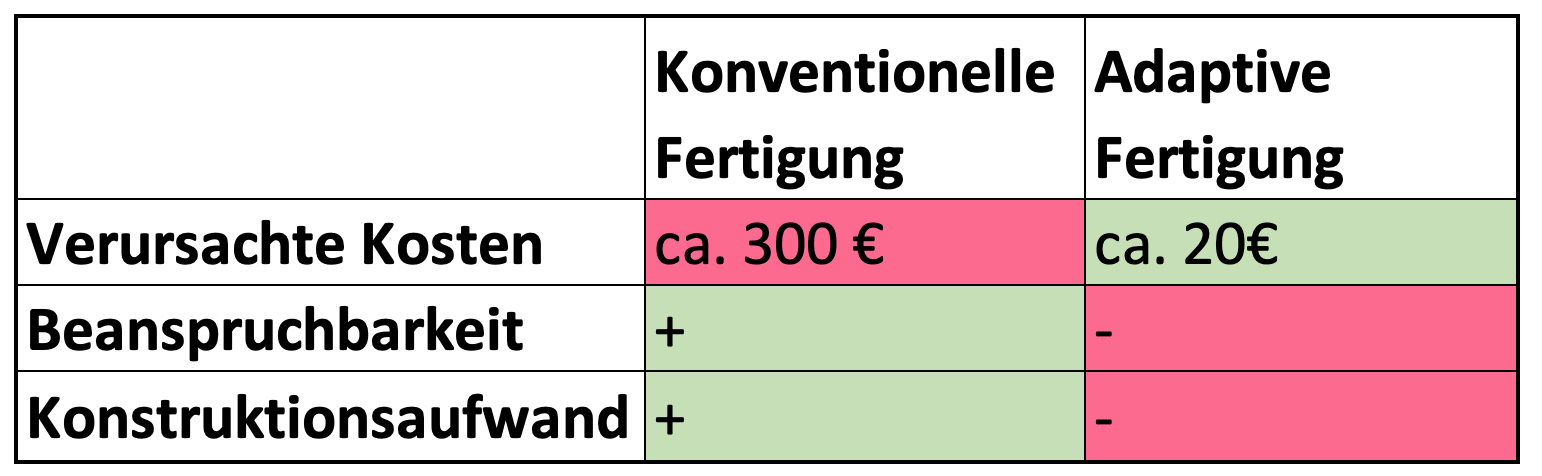
\includegraphics[width=12cm]{fertigungsverfahren.png}
%	\caption{Konstruktionsansicht der verschiebbaren Motoraufhängung}
%	\label{pic:fertigungsverfahren}
%\end{figure}
%
%
%Aufbereitungs-  Rüstzeit 
%
%Bei hoch beanspruchten Teilen: Konventionelle Fertigungsverfahren 
%Aufwändige Konturen: Adaptive Fertigung
%
%
%	


%-------------------------FAZIT UND AUSBLICK-----------------


\chapter{Fazit und Ausblick}
In diesem ersten Teil der Studienarbeit wurden zunächst Grundlagen geschaffen und Anforderungen an die digitalisierte Version der Hochbahn gestellt. Anschließend wurden die Konzepte zum Erreichen der Forderungen erstellt. Im Teil der Umsetzung wurden bereits erste Versuche durchgeführt und Prototypen getestet.\\

Im weiteren Verlauf der Arbeit gilt es nun, die Umsetzung weiter fortzuführen. Dabei steht vor allem die Fertigung der beschriebenen Bauteile an. Anschließend können die informationstechnischen Anwendungen erstmals zusammen mit dem Aufbau getestet werden. Diese Vorhaben sollen vor allem in der folgenden Praxisphase umgesetzt werden. 